\documentclass[superscriptaddress,floatfix,reprint,prl]{revtex4-1}
\usepackage{epsfig,hyperref,graphics,float,amsmath,mathtools}
\usepackage{microtype,setspace,physics,epsfig,graphicx,amssymb}
\usepackage[caption=false]{subfig}
\usepackage[per-mode=symbol]{siunitx}
\usepackage{xcolor}
\usepackage{nameref}
\captionsetup[subfigure]{labelformat=brace}
\definecolor{matplotlibBlue}{HTML}{1F77B4}
\definecolor{matplotlibOrang}{HTML}{FF7F0E}

\begin{document}
\bibliographystyle{apsrev4-1}


\title{A Chiral, Incommensurate Helical Phase in a Smectic of Achiral Bent-Core Mesogens}
\date{\today}
\author{Adam A.~S.~Green}
\affiliation{Department of Physics and Soft Materials Research Center,
University of Colorado Boulder, Boulder, CO, 80309-0390, USA}
\author{Michael R.~Tuchband}
\affiliation{Department of Physics and Soft Materials Research Center,
University of Colorado Boulder, Boulder, CO, 80309-0390, USA}
\author{Renfan Shao}
\affiliation{Department of Physics and Soft Materials Research Center,
University of Colorado Boulder, Boulder, CO, 80309-0390, USA}
\author{Yongqiang Shen}
\affiliation{Department of Physics and Soft Materials Research Center,
University of Colorado Boulder, Boulder, CO, 80309-0390, USA}
\author{Rayshan Visvanathan}
\affiliation{Department of Physics and Soft Materials Research Center,
University of Colorado Boulder, Boulder, CO, 80309-0390, USA}
\author{Alexandra~E.~Duncan}
\affiliation{Department of Physics and Soft Materials Research Center,
University of Colorado Boulder, Boulder, CO, 80309-0390, USA}
\author{Anne Lehmann}
\affiliation{Department of Chemistry, Martin Luther University
Halle-Wittenberg, D-06120 Halle, Germany}
\author{Carsten Tschierske}
\affiliation{Department of Chemistry, Martin Luther University
Halle-Wittenberg, D-06120 Halle, Germany}

\author{Eric D.~Carlson}
\affiliation{Department of Chemistry and Soft Materials
Research Center,
University of Colorado Boulder, Boulder, CO, 80309-0215, USA}
\author{Edward Guzman}
\affiliation{Department of Chemistry and Soft Materials
Research Center,
University of Colorado Boulder, Boulder, CO, 80309-0215, USA}
\author{Maria Kolber}
\affiliation{Department of Chemistry and Soft Materials
Research Center,
University of Colorado Boulder, Boulder, CO, 80309-0215, USA}
\author{David M.~Walba}
\affiliation{Department of Chemistry and Soft Materials
Research Center,
University of Colorado Boulder, Boulder, CO, 80309-0215, USA}

\author{Cheol S.~Park}
\affiliation{Department of Physics and Soft Materials Research Center,
University of Colorado Boulder, Boulder, CO, 80309-0390, USA}
\author{Matthew A.~Glaser}
\affiliation{Department of Physics and Soft Materials Research Center,
University of Colorado Boulder, Boulder, CO, 80309-0390, USA}

\author{Joseph E.~Maclennan}
\affiliation{Department of Physics and Soft Materials Research Center,
University of Colorado Boulder, Boulder, CO, 80309-0390, USA}

\author{Noel A.~Clark}
\affiliation{Department of Physics and Soft Materials Research Center,
University of Colorado Boulder, Boulder, CO, 80309-0390, USA}


\newcommand{\jem}[1]{{{\color{black} #1}}}

\begin{abstract}
An achiral, bent-core mesogen forms several tilted smectic liquid crystal phases,
including a non-polar, achiral de Vries smectic A which transitions to a chiral,
ferroelectric state in applied electric fields above a threshold.  At lower
temperature, a chiral, ferrielectric phase with a periodic, supermolecular modulation of
the tilt azimuth, indicated by a Bragg peak in carbon-edge resonant soft
X-ray scattering, is observed. The absence of a corresponding resonant Umklapp peak
identifies the superlayer structure as a twist-bend-like helix that is only weakly
modulated by the smectic layering.
\end{abstract}


\newcommand{\smapr}[1]{$\mathrm{SmAP}_\mathrm{R}$}
\newcommand{\sma}[1]{$\mathrm{SmA}$}
\newcommand{\smapf}[1]{$\mathrm{SmAP}_\mathrm{F}$}
\newcommand{\smapa}[1]{$\mathrm{SmAP}_\mathrm{A}$}
\newcommand{\smcapalp}[1]{$\mathrm{SmC}_\textrm{A}\textrm{P}_\mathrm{\alpha}$}
\newcommand{\smapalp}[1]{$\mathrm{SmAP}_\mathrm{\alpha}$}
\newcommand{\smcapf}[1]{$\mathrm{SmC}_\textrm{A}\textrm{P}_\mathrm{F}$}
\newcommand{\smcspf}[1]{$\mathrm{SmC}_\textrm{S}\textrm{P}_\mathrm{F}$}
\newcommand{\smcspa}[1]{$\mathrm{SmC}_\textrm{S}\textrm{P}_\mathrm{A}$}
\newcommand{\smchph}[1]{$\mathrm{Sm(CP)}_\alpha$}

\newcommand{\smarprM}[1]{\text{de Vries SmA}}
\newcommand{\smarpr}[1]{$\text{de Vries SmA}$}

\newcommand{\smchphM}[1]{\mathrm{Sm(CP)}_\textrm{s3}}
\newcommand{\smcdpd}[1]{$\mathrm{SmC}_\textrm{D}\textrm{P}_\mathrm{D}$}
\newcommand{\smcdpdM}[1]{\mathrm{SmC}_\textrm{D}\textrm{P}_\mathrm{D}}
\newcommand{\smcapa}[1]{$\mathrm{SmC}_\textrm{A}\textrm{P}_\mathrm{A}$}
\newcommand{\smcapaprime}[1]{$\mathrm{SmC}_\textrm{A}\textrm{P}_\mathrm{A'}$}
\newcommand{\smaprM}[1]{\mathrm{SmAP}_\mathrm{R}}
\newcommand{\smaM}[1]{\mathrm{SmA}}
\newcommand{\smapfM}[1]{\mathrm{SmAP}_\mathrm{F}}
\newcommand{\smapaM}[1]{\mathrm{SmAP}_\mathrm{A}}
\newcommand{\smapalpM}[1]{\mathrm{SmAP}_\mathrm{\alpha}}
\newcommand{\smcapfM}[1]{\mathrm{SmC}_\textrm{A}\textrm{P}_\mathrm{F}}
\newcommand{\smcspfM}[1]{\mathrm{SmC}_\textrm{S}\textrm{P}_\mathrm{F}}
\newcommand{\smcspaM}[1]{\mathrm{SmC}_\textrm{S}\textrm{P}_\mathrm{A}}
\newcommand{\smcapaM}[1]{\mathrm{SmC}_\textrm{A}\textrm{P}_\mathrm{A}}

\newcommand{\smcapaprimeM}[1]{\mathrm{SmC}_\textrm{A}\textrm{P}_\mathrm{A`}}

\newcommand{\nsix}[1]{\textbf{n-16}}
\newcommand{\nfour}[1]{\textbf{PAL30}}
\newcommand{\smcp}[2]{SmC$_\text{#1}$P$_\text{#2}$}
\newcommand{\smap}[1]{SmAP$_\text{#1}$}

\maketitle
The discovery of spontaneous macroscopic polar
ordering~\cite{niori_distinct_1996} and chirality~\cite{link_spontaneous_1997} in
fluid smectic liquid crystal phases of achiral  bent-core mesogens has led to
the exploration of a rich family of novel liquid crystal phases and
self-assemblies~\cite{takezoe_bent-core_2006,eremin_polar_2013,takezoe2017bent,chattham_triclinic_2010,reddy_spontaneous_2011}
 in which the key macroscopic elements of polarity, chirality, and smectic layering all appear as spontaneously broken symmetries.
While the smectic layer-scale order of bent-core mesogens, resulting from strong intralayer
coupling between molecular tilt and polarity, is quite well characterized, superlayer
structuring beyond that of the four basic SmCP bilayer phases combining synclinic or
anticlinic tilt with ferroelectric or antiferroelectric
polarity~\cite{link_spontaneous_1997}, as sketched in Supplemental Figure~S1, have
not been definitively identified.
Possible superlayer structures analogous to those seen in tilted SmC*
phases of chiral, rod-shaped molecules could be incommensurate or commensurate with the
underlying smectic layer spacing and feature states of varying azimuthal orientation
of the molecular long axis about the layer normal, $z$, such as the chiral
helical precession along $z$ with equal, discrete orientational jumps between layers of
the $\mathrm{SmC}^*_\alpha$ phase and the ferrielectric phases with periodic arrays of discrete jumps of
different sizes~\cite{takezoe2010antiferroelectric}.

Since the period of such superlayer structures, $p$,  can be as short as two
layers, the structural study of such phases requires the
effective probing of molecular orientation at the nanoscale. This can be
achieved using resonant X-ray scattering, a technique sensitive to atomic
environment~\cite{mach_structural_1998,levelut1999tensorial,mach_structures_1999,hirst2002interlayer,gleeson_resonant_2006,Barois2012review,folcia2014spontaneous,huang2015liquid,zhu2015probing,zhu2016resonant,salamonczyk2017structure}
that has previously enabled the discovery and
definitive characterization of superlayer organization in several SmC* phases and sub-phases, employing
the K-edge resonance of atoms incorporated in the liquid crystal molecule~\cite{mach_structural_1998,mach_structures_1999}.

Several recent
observations suggest the possibility of chiral superlayer ordering in achiral
bent-core mesogens: Takanishi et al.\ have identified such a structure in a
SmCP phase of a bent-core mesogen doped with a chiral, rod-shaped molecule that as a neat
material exhibits $\mathrm{SmC}^*_\alpha$ and ferrielectric phases~\cite{takanishi2015chiral};
Abberley et al.\ have reported a superlayer helix in a smectic phase of bent dimers of molecular
rods~\cite{abberley2018heliconical}; Panarin and co-workers have recently proposed,
based on AFM
evidence, the existence of tilted, helical supermolecular ordering in several achiral bent-core mesogens with $4$-cyanoresorcinol bisbenzoate cores~\cite{sreenilayam_spontaneous_2016}.
Earlier investigations of this molecular family had concluded, however, that their polar phases were orthogonal, i.e.,  untilted and therefore not chiral~\cite{panarin_sequence_2011,sreenilayam_properties_2012}.
Motivated by these conflicting reports and the ongoing interest in the chiral sub-phases of liquid crystals, we have studied one of the members of this
homologous series, \nfour{phi}, which has $n = 14$ alkyl tails (see Figure~\ref{fig:main}(a)). Our experiments, using
non-resonant X-ray scattering (SAXS), resonant soft X-ray scattering (RSoXS), electro-optic techniques, and polarized light
microscopy (PLM), summarized in Figure~\ref{fig:main}, reveal an exotic phase sequence, including
an achiral de Vries smectic which becomes chiral in sufficiently large applied
electric fields, and, at lower temperature, a tilted, chiral smectic with superlayer helical
ordering.

\begin{figure*}
    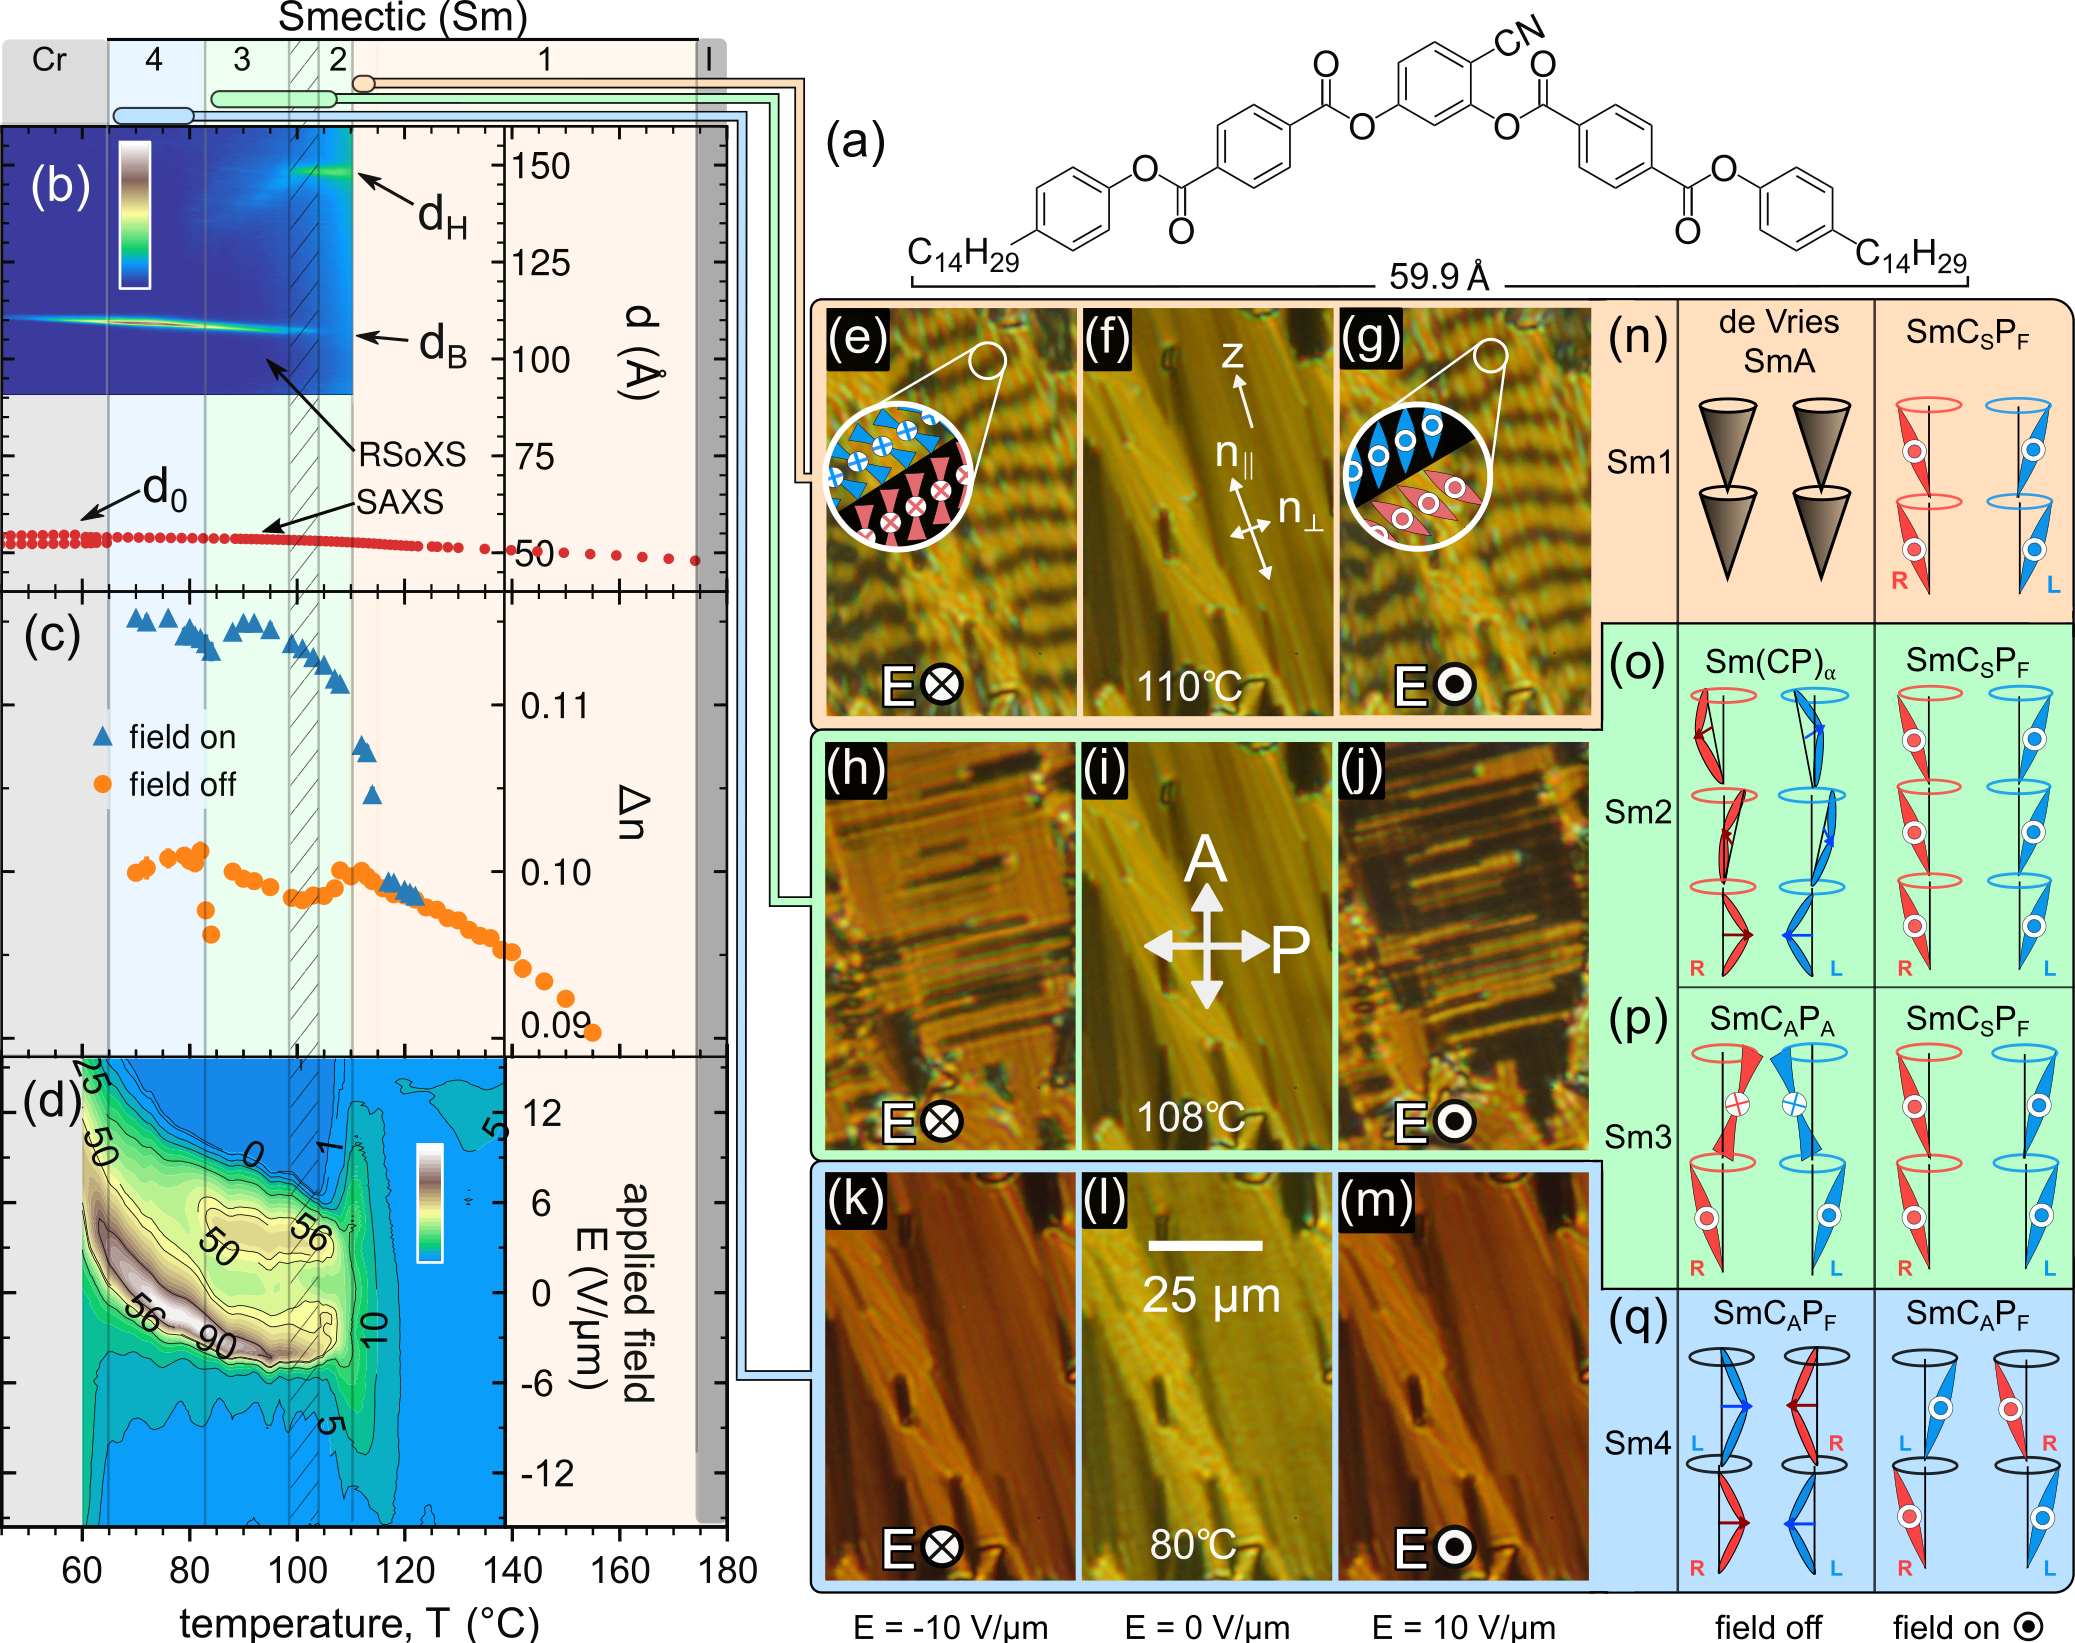
\includegraphics[width=2\columnwidth]{Figure1v3.png}
    \caption{\label{fig:main}
        Experimental characterization of \nfour{phi}. (a) The \nfour{phi} molecule, showing the
        all-trans length calculated using the program Spartan. (b--d) Phase properties vs.\ temperature. The solid vertical lines denote phase boundaries and the cross-hatching phase coexistence.
    (b) SAXS shows the smectic layer spacing in all
    phases to be $d_0 \approx \SI{48}{\angstrom}$. Resonant carbon K-edge
    reflections are from superlayer
    modulations of the molecular orientation about the layer normal $z$, the peak
    at $d_H \approx \SI{150}{\angstrom}$ corresponding to the pitch of the incommensurate, helical precession in the Sm2 phase, and at
    $d_\text{B}=2d_0$ to the bilayer ordering of the Sm3 and Sm4 phases.
    (c) Birefringence of planar-aligned cells with layers normal to the plates, with and without applied electric
    field ($E = \SI{20}{\volt\per\micro\metre}$).
    (d) Polarization current (in nA) in response to a triangle-wave applied electric field:
    a single-peak, Langevin-like response at lower
    temperatures in the Sm1
    phase; a triple peak in the Sm2 phase, associated with ferrielectric
    switching\cite{findeisen2008multistage} and indicative of helical
    unwinding\cite{takezoe2010antiferroelectric}, coalescing into a double peak in the Sm3, indicating a
    non-polar ground state at $E = 0$; and a single current peak in the Sm4 phase
    caused by the block polarization switching of the ferroelectric \smcapf{phi} ground state.
    (e--m) Characteristic optical textures in a planar cell, viewed between
    crossed polarizers. The $E = 0$ textures are
    focal conics typical of a fluid smectic with an optic axis along $z$.
    Field application induces chiral, tilted conglomerate domains (of opposite
    handedness) in the Sm1--Sm3 phases, but only a
    change in birefringence in the Sm4.
    (n--q) Proposed superlayer structure of \nfour{phi} phases, with and without
    applied electric field: (n) Sm1: achiral de Vries-like SmA
    $\rightarrow$ chiral \smcspf{phi};  Sm2: superlayer chiral helix
    $\rightarrow$ chiral \smcspf{phi}; Sm3: superlayer chiral bilayer
    \smcapa{phi} $\rightarrow$ chiral \smcspf{phi}; Sm4: \smcapf{phi} with
    $\textbf{P}$ parallel to the glass $\rightarrow$ \smcapf{phi}
    with $\textbf{P}$ normal to the glass.
            }
\end{figure*}

X-ray scattering from \nfour{phi} is shown in Figures~\ref{fig:main}(b) and S3.
Upon  cooling from the isotropic, a single, non-resonant SAXS peak
appears at $\SI{175}{\degreeCelsius}$, at a wavevector $q_0$  corresponding to Bragg scattering from
the smectic layers in the Sm1 phase with spacing $d_0 = 2\pi/q_0
= \SI{48}{\angstrom}$. The layer spacing increases slightly on cooling
to the crystal phase at \SI{65}{\degreeCelsius} and is
consistently smaller than the calculated molecular length, $l = \SI{59.9}{\angstrom}$, throughout this temperature range, suggesting that the molecules are tilted in all of the smectic phases, to first order by an average amount estimated using $\theta_\textrm{xray} =
\cos(d_0/l)$ of $\SI{33}{\degree}$ (see Figure~S4).
In the Sm1 temperature range ($\SI{110}{\degreeCelsius} \leq T \leq
\SI{175}{\degreeCelsius}$), there are no RSoXS scattering features that would indicate a
superlayer periodic structure (see Figure~S2 and the Supplemental video).

At the transition to the Sm2 phase, at $\SI{110}{\degreeCelsius}$, marked  by
a distinct enthalpy peak in the DSC (Figure~S5
), a single, sharp
resonant peak appears at $q_H = \SI[per-mode=reciprocal]{.042}{\per\angstrom}$, corresponding
to a molecular orientational structure with a period
$d_H=\SI{148}{\angstrom}\approx 2.8 d_0$ that is incommensurate with the
smectic layer spacing (Figure~\ref{fig:xray-results}(b)). Below
$\SI{104}{\degreeCelsius}$, this reflection
becomes weaker and another sharp, resonant reflection at higher $q$ grows in, the coexistence
indicating a first-order transition to the Sm3 phase.
This second Bragg peak, which persists down to the crystal phase, has a
wavevector $q_B\approx q_0/2$, indicative of a commensurate, bilayer orientational
structure in the Sm3 and Sm4 phases.
%
Below \SI{99}{\degreeCelsius}, the incommensurate peak broadens dramatically and
moves to higher $q$, indicating the presence of short-ranged, Sm2-like helical
fluctuations persisting in the Sm3 phase, and disappears at the transition to the Sm4
phase at \SI{83}{\degreeCelsius}. The Sm4 phase exhibits only the bilayer RSoXS
reflection at $q_B$.

\begin{figure}
    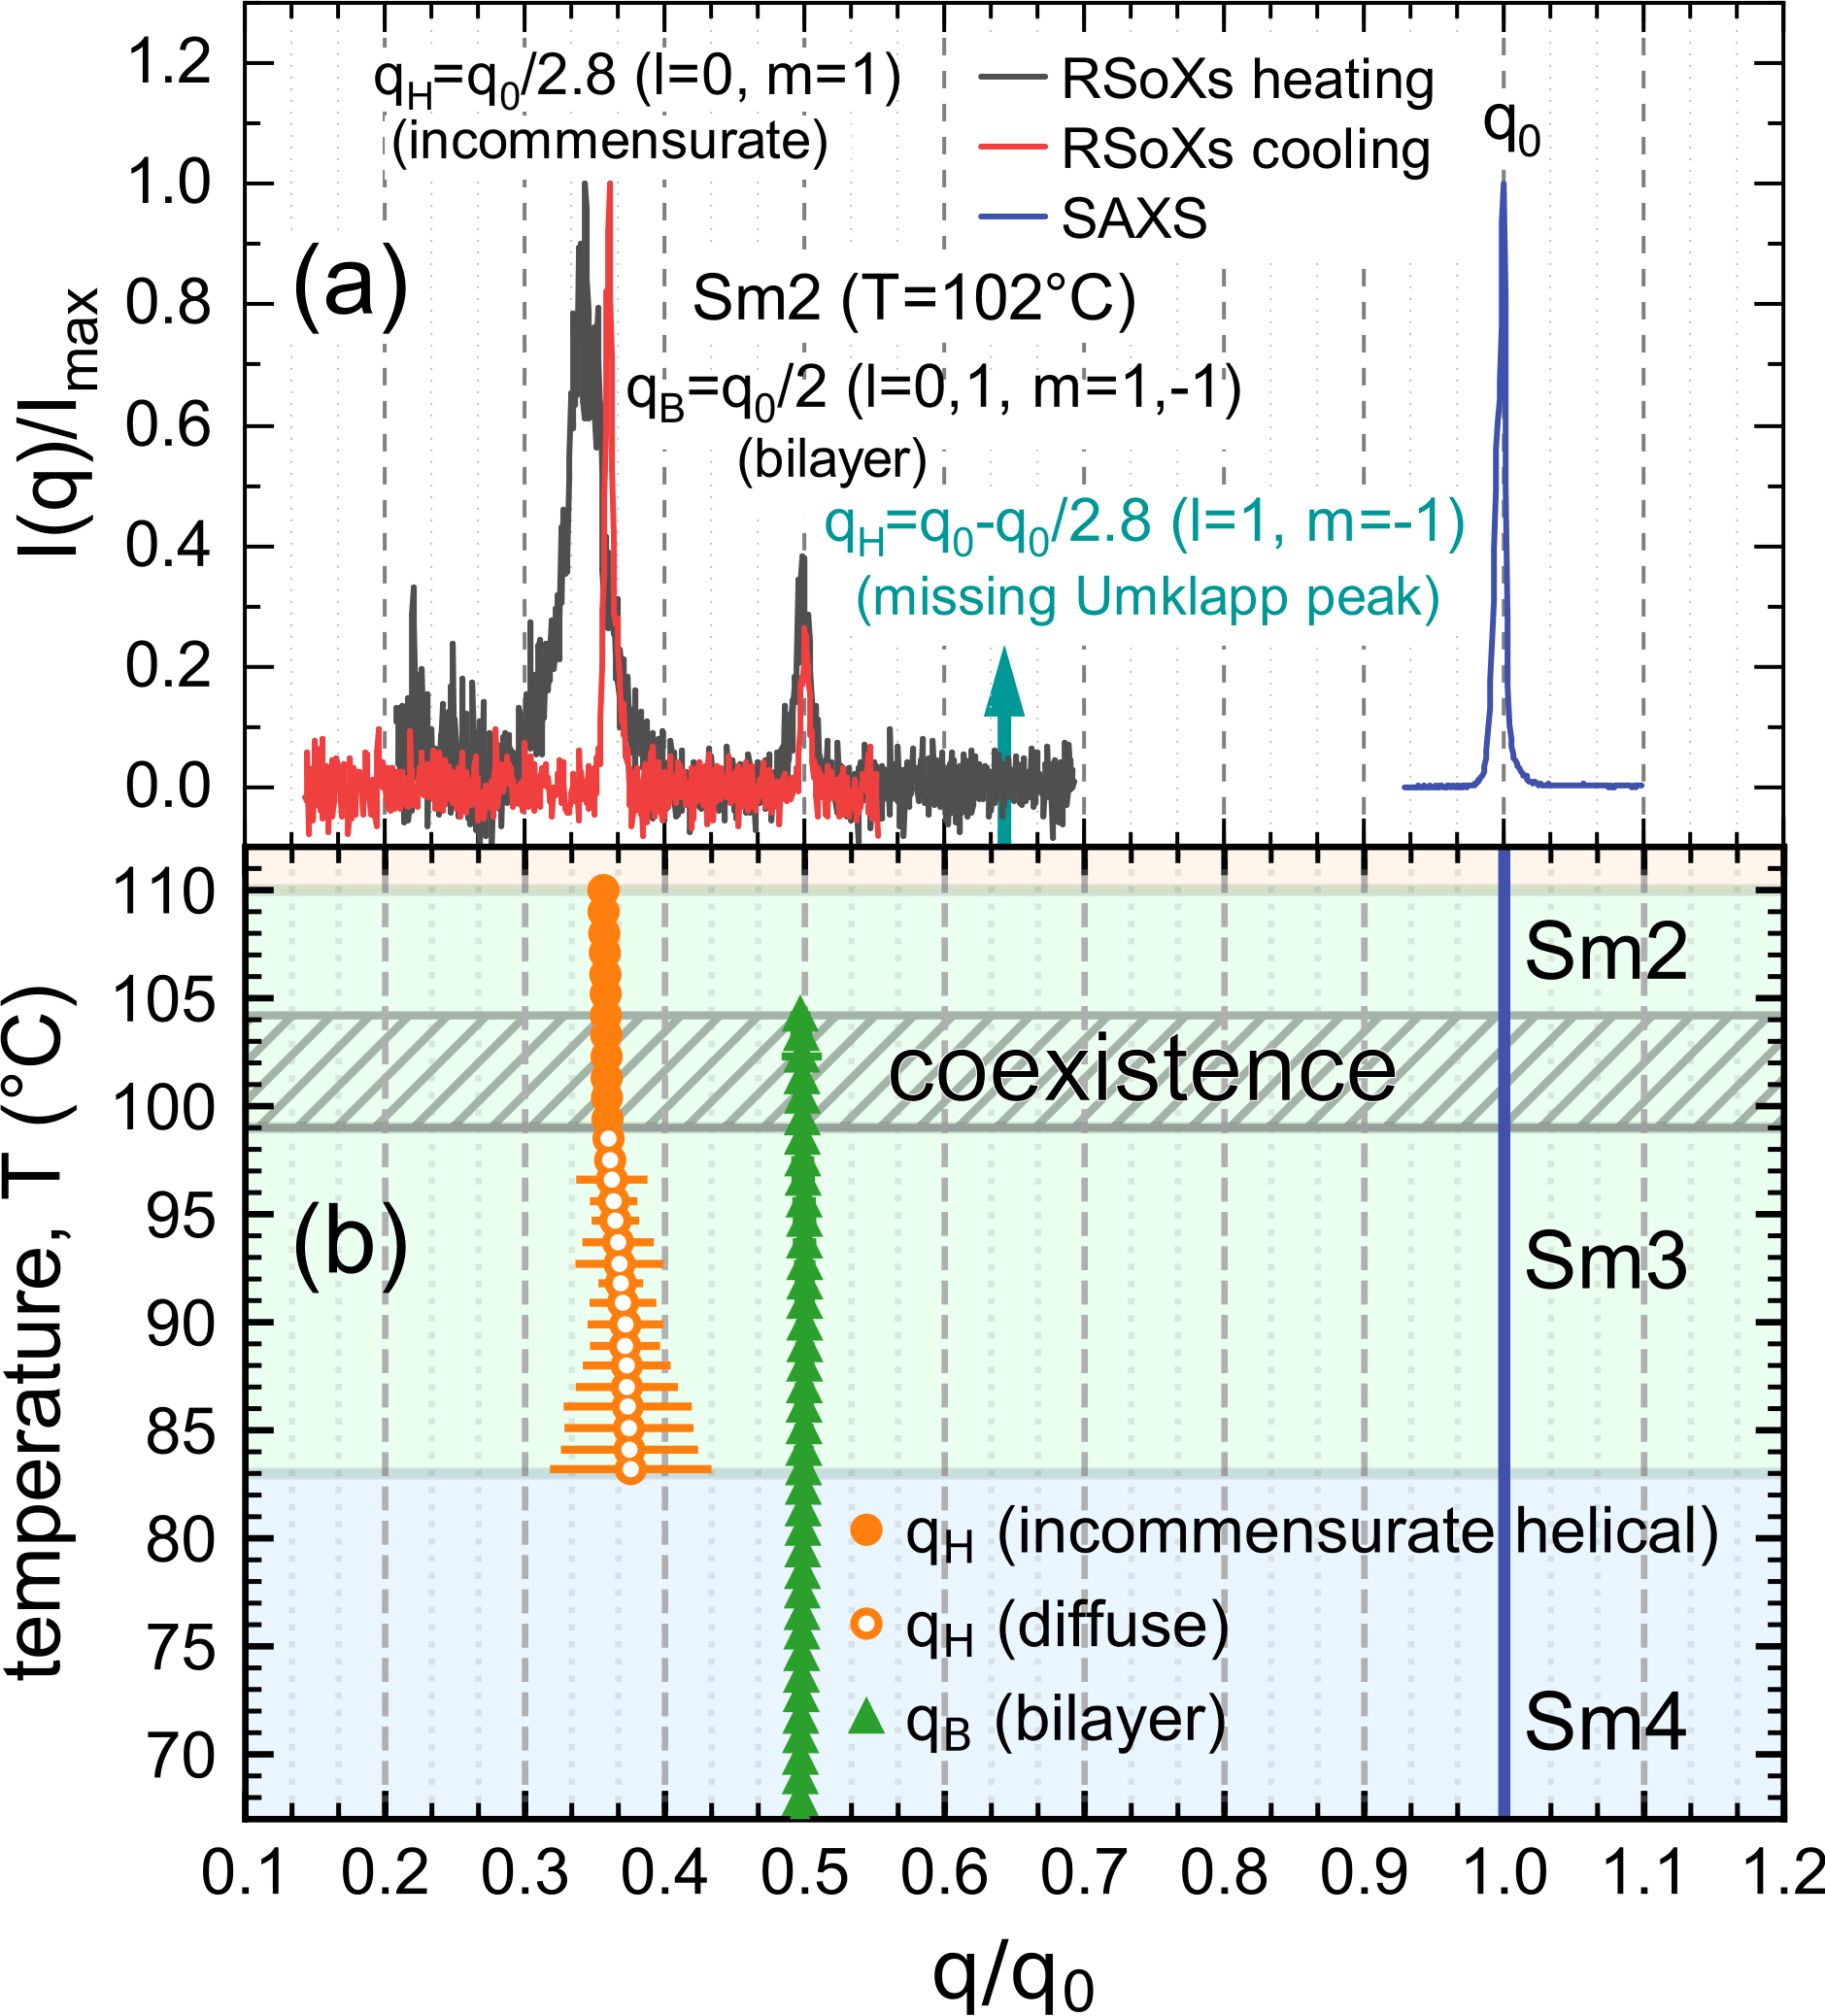
\includegraphics[width=\columnwidth]{xray-combined.png}
    \caption{\label{fig:xray-results}X-ray scattering from \nfour{phi}.
        (a) SAXS gives a peak from the smectic layer ordering at $q=q_0$.
        The RSoXS peak at $q_H$ indicates that there is superlayer orientational ordering with periodicity $d_H$
        in the Sm2 phase.
        In general, superlayer orientational modulation in a smectic generates RSoXS peaks at wavevectors along the layer normal at
        $q(l,m) = l(2\pi/d_0) \pm m(2\pi/d_H)$\cite{levelut1999tensorial}.  The
        observation of an RSoXS reflection at $q = q(0,1)$ and the absence of an Umklapp peak at $q = q(1,-1)$  in
        the Sm2 confirms a superlayer helix with a scattering amplitude
        modulation due to the smectic layering that is undetectably weak.
        (b) Temperature dependence of resonant scattering. The helix peak at $q_H \approx1/(2.8 d_0)$ becomes diffuse in the Sm3 phase. Splitting
        of the bilayer peak at $q_B$, which would indicate helical precession of the bilayer structure, is not observed.
        }
\end{figure}


The RSoXS scattering from a single layer can be analyzed, following Levelut and
Pansu, in terms of a monoclinic second-rank tensor with a principal
axis tilted from and then azimuthally rotated about the layer normal~\cite{levelut1999tensorial,gleeson_resonant_2006,Barois2012review}.   Scattering
from a stack of such layers is calculated by summing over the contributions of the individual layers at different $z$.
Resonant scattering peaks from azimuthally
periodic arrangements are found at wavevectors along $z$, $q(l,m) = l(2\pi/d_0)
\pm m(2\pi/p)$, where $p$ is the pitch.  In principle, resonant
scattering should appear at all values of $l$ (harmonics of $q_0$), and at values
of $m=0,\pm1,\pm2$ that depend on the superlayer structure.  In an incommensurate, helical
structure, like the SmC$_\alpha$ phase, only the fundamental and harmonic peaks at
$q(l=0,m=+1,+2)$ and the Umklapp peaks at
$q(l=+1,m=-1,-2)$ are found in the range $0 < q(l,m) <
q_0$. If the resonant scatterers are confined to lie precisely on layers spaced
by $d_0$, then the intensities of these peaks will be identical~\cite{levelut1999tensorial}.
Out-of-layer molecular positional fluctuations, and, in particular,
those for which there is a coupled azimuthal orientation that keeps the molecule
on the helix, $\delta \phi = (2\pi/p)\delta z$, reduce the intensities of the
resonant harmonic peak
at $2q_H$ and of the Umklapp peaks at $q_0 \pm q_H$, relative to that of the fundamental at
$q_H$~\cite{levelut1999tensorial}. In our RSoXS scans of these peaks, only the
fundamental is seen above the background, so that only the upper limit of
the intensity ratio of the Umklapp and fundamental peaks
can be estimated. From the RSoXS heating scan of
Figure~\ref{fig:xray-results}(a), we find $I_\text{U}/I_\text{F} \alt 0.03$, implying a very
weak fractional modulation of the density of helical scatterers, $\rho$, due to fluctuations in the
smectic layering $\sqrt{\langle\delta\rho^2\rangle}/\rho_0 < 0.17$. The absence of the harmonic peaks places a similar limit on how much the density modulation of helical scatterers deviates from being purely sinusoidal.

The optical textures of planar-aligned (bookshelf) cells of
\nfour{phi} were studied using PLM.
Upon cooling from the isotropic, the Sm1 phase grows in (at \SI{175}{\degreeCelsius})
as b\^{a}tonnets, giving a smooth, focal-conic texture typical of an orthogonal fluid smectic (Figure~\ref{fig:main}(f)).
However, given the large value of the estimated
molecular tilt, $\theta_\textrm{xray}$, the Sm1 is probably a de Vries
smectic.
In planar-aligned cells, there is no observable field-induced change of the in-plane birefringence, $\Delta n= n_\parallel
-n_\perp$, in small applied electric fields  (Figure~\ref{fig:main}(f)),
or in the optic axis orientation, $\theta_\text{opt}$ (Figure~\ref{fig:threshold}).

Below \SI{115}{\degreeCelsius}, a threshold field, $E_\text{th}$, above which a first-order structural change marked by the appearance of chiral conglomerate domains occurs, becomes experimentally accessible.
These domains are polar and exhibit a uniform, saturated optic axis tilt on the
order of $\theta_{\rm opt} \approx \SI{18}{\degree}$ from the layer normal, implying that the achiral, untilted Sm1 phase
transforms in the field to a B2-like, homochiral \smcspf{phi} state (Figure
S1(c))~\cite{eremin2008electrically}. The field-induced left- and right-handed domains form a ``tiger stripe''
pattern (Figures~\ref{fig:main}(e,g)). The local domain handedness in this unusual conglomerate texture
is apparently locked in after the first few field cycles.  This bias is due to a chiral
memory effect at the surface since, as
Figures~\ref{fig:main}(d)~and~\ref{fig:threshold} show, the
sub-threshold bulk state has an achiral field response, with a linear polarization current (implying $P \propto E$) and no
detectable reorientation of the optical tilt.
$E_\text{th}$  decreases strongly on cooling as the transition to the Sm2 phase is approached, as shown in the inset of Figure~\ref{fig:threshold}.
%
\begin{figure}[h]
    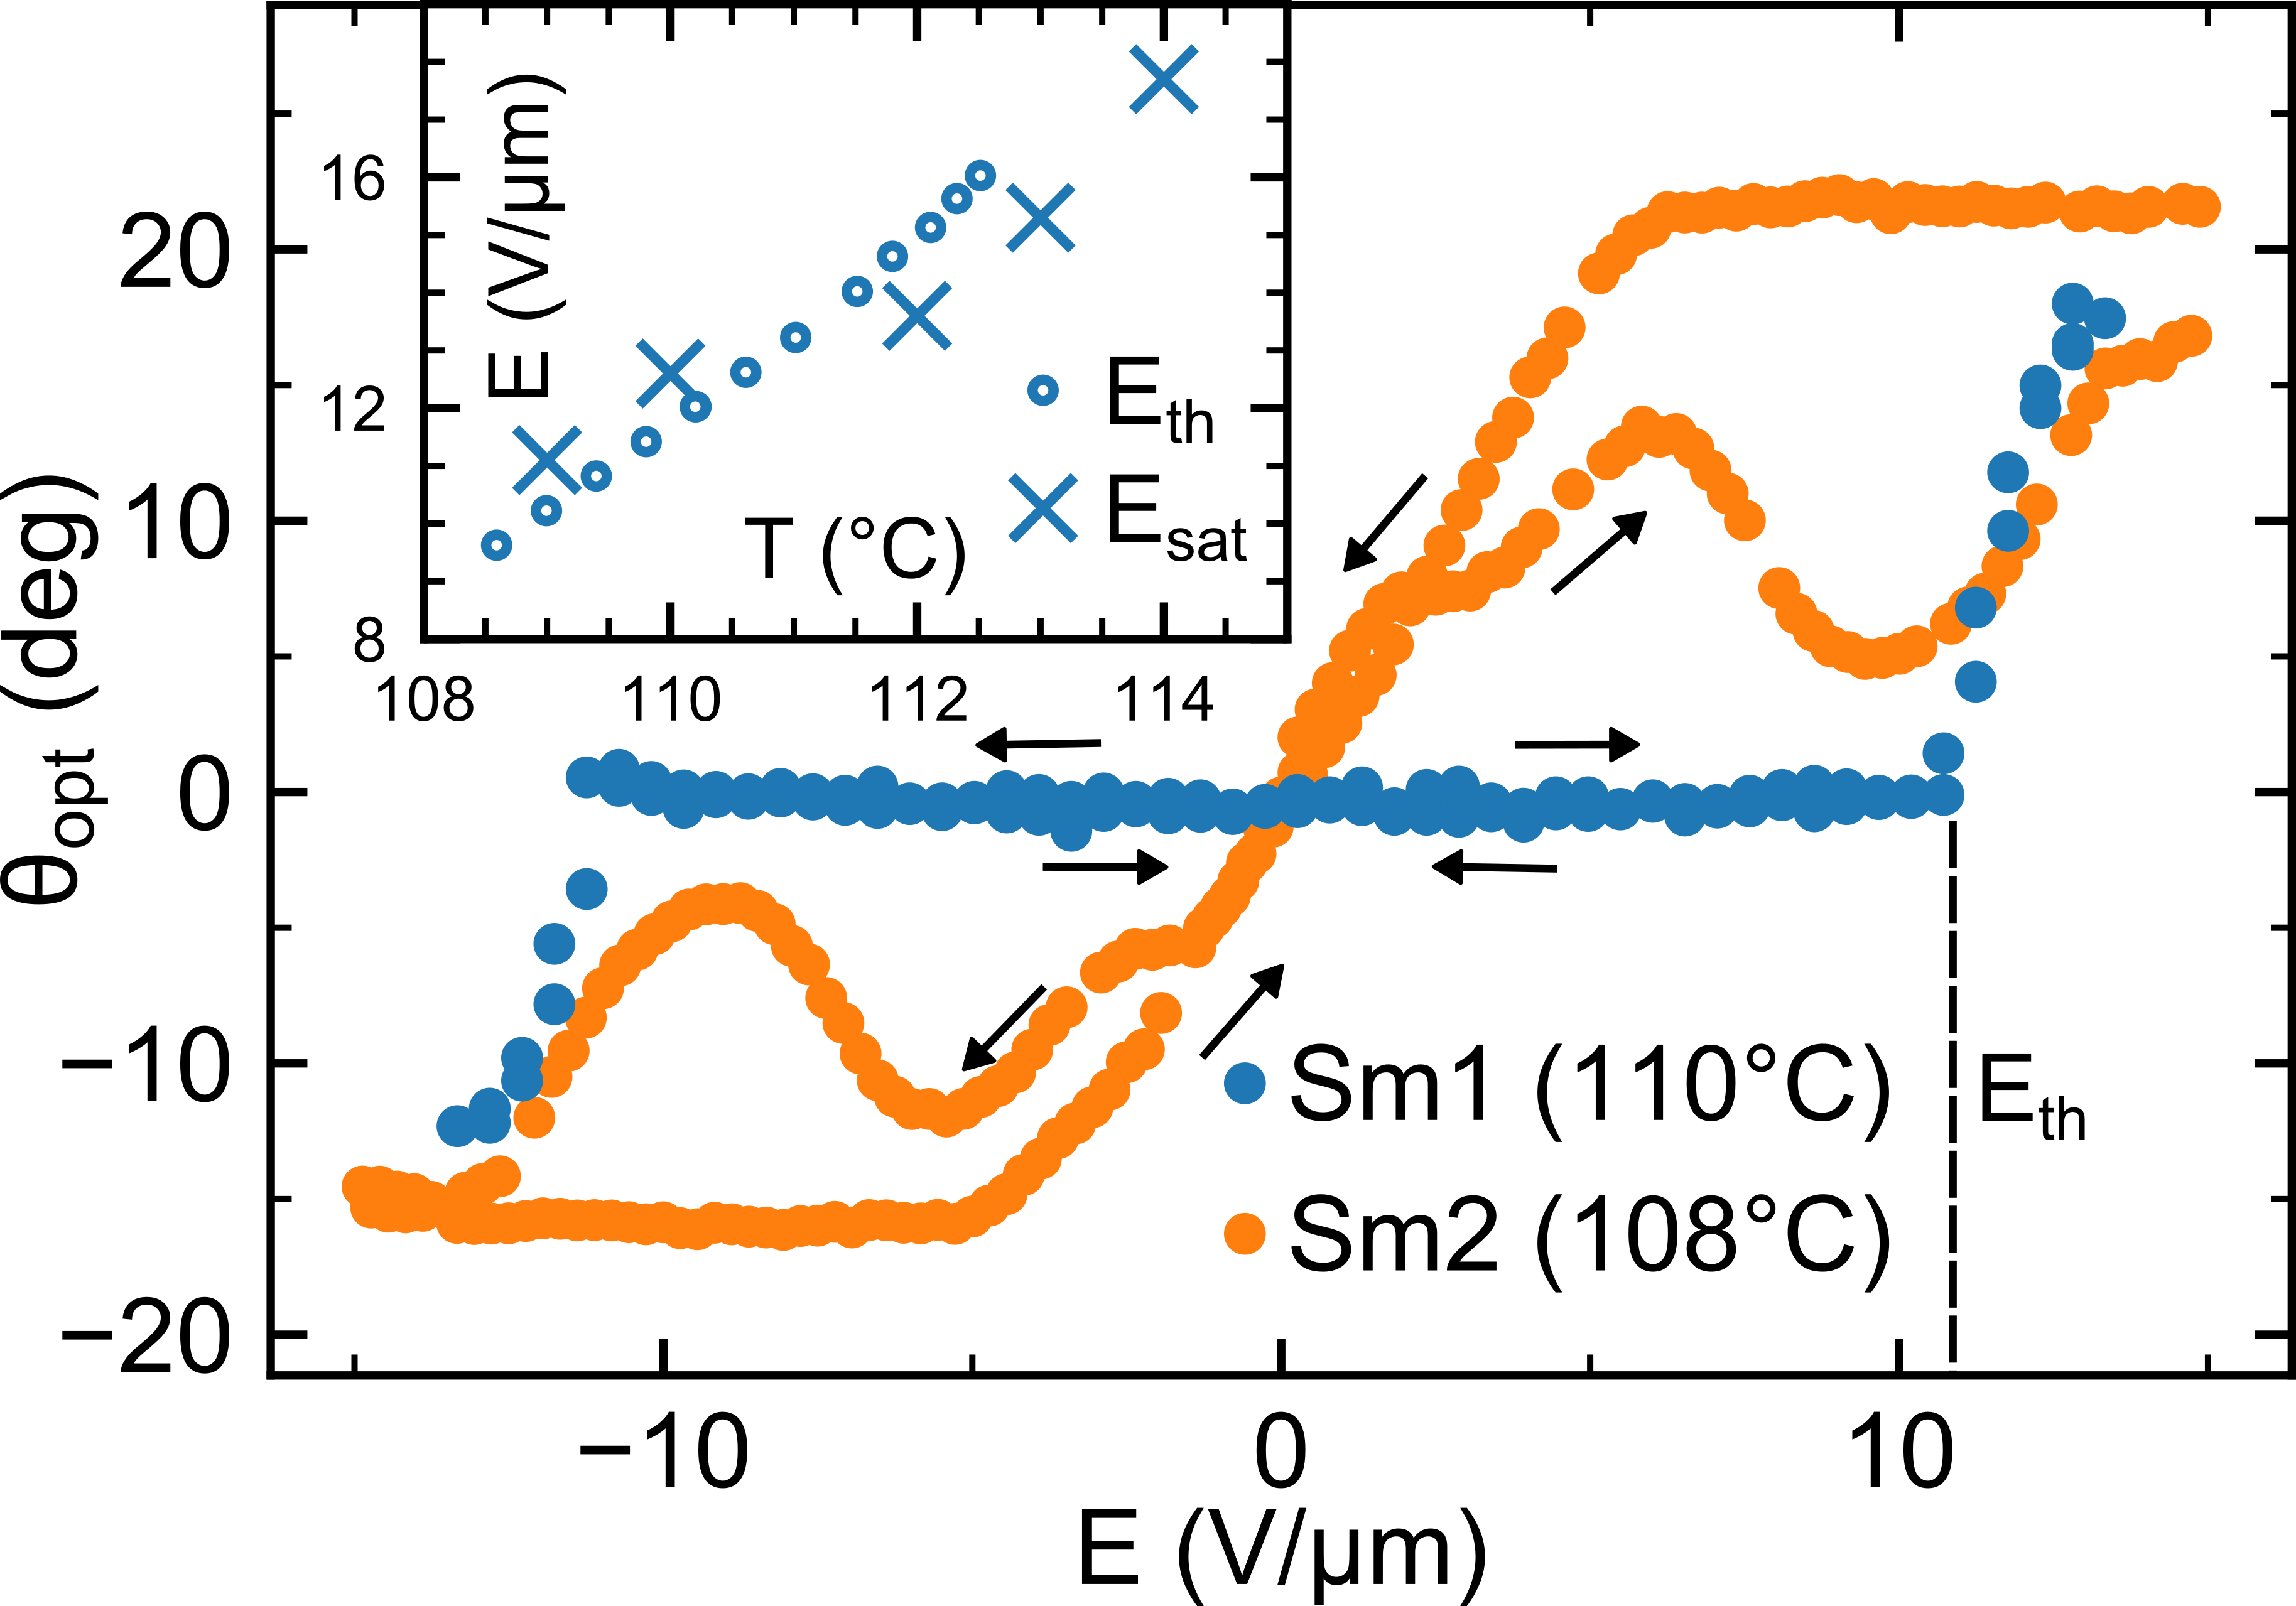
\includegraphics[width=\columnwidth]{threshold-inset2.png}
    \caption{\label{fig:threshold}
        Optical tilt of \nfour{phi} vs.\ applied field. The Sm1
        phase shows no electrooptic response in weak fields $E<E_\text{th}$. Fields $E>E_\text{th}$ induce an electroclinic
        tilt and result in the formation of chiral domains.
        $E_\text{th}$, which becomes smaller with decreasing $T$ (inset), matches
        closely $E_\text{sat}$, the field at which the induced
        polarization saturates, extracted from Figure~\ref{fig:main}(d).
        The Sm2 phase exhibits a chiral
        electroclinic effect near $E=0$ and hysteresis in the field-induced helix unwinding to the
        \smcspf{phi} state.   }

\end{figure}


In the lower part of the Sm1, and throughout the Sm2, Sm3 and Sm4 phases, the birefringence increases on application of an electric field, as seen in Figure~\ref{fig:main}(c),  changing from yellow to orange.
Measurements of $\Delta n$ at $E = 0$ and $E = \SI{20}{\volt\per\micro\metre}$
(Figures~\ref{fig:main}(c) and S6),
show that the birefringences in the lower temperature
phases with and without an applied field are of the order of $\Delta n_\text{on} \sim 0.12$ and $\Delta n_\text{off} \sim 0.10$.
Assuming that the field-on \smcspf{phi} state
(Figures~\ref{fig:main}(n--p) and S1) gives a uniform
director orientation with the optic axis in the plane of the cell, then $\Delta
n \sim 0.12$ would correspond to the maximal birefringence $n_3-n_1$ of the
\smcspf{phi} state. Modeling the bent-core molecule
as two uniaxial, birefringent rods connected with an opening angle of
$\Psi$, and tilting this molecule from $z$ by an angle $\theta$,
we have calculated the birefringence of all of the states shown in
Figure~\ref{fig:main}. If the Sm1 phase is assumed to be a de Vries SmA, with
azimuthally averaged molecules distributed on a tilt cone of angle
$\theta$, the best fit to the measured birefringence values $\Delta n_\text{on}$ and $\Delta n_\text{off}$ is
obtained with $\Psi = \SI{150}{\degree}$ and $\theta = \SI{15}{\degree}$.
The calculated birefringence as a function of temperature is shown in Figure~S6.



The transitions between the smectic phases are difficult to see when $E=0$ because they are all orthogonal in appearance,
with an optic axis along $z$, and have similar birefringence.
At the transition from Sm1 to the Sm2 phase,  however, arbitrarily small electric fields induce molecular tilt in the
(Figure~\ref{fig:threshold}), leading to the formation of optically distinct, conglomerate chiral
domains with opposite tilt (Figures~\ref{fig:main}(h--j)), again
corresponding to a field-induced transition to a \smcspf{phi} state.
The birefringence and orthogonal appearance of the Sm2 ground state are consistent with
the helical superlayer structure indicated by RSoXS.

The texture and birefringence of the Sm3 phase in the absence of field are consistent with the \smcapa{phi} bilayer structure indicated by RSoXS.
The field-induced conglomerate domain morphology in both the Sm2 and Sm3 phases is distinct from that of the undulating Sm1
tiger stripes, with straight
domain boundaries that tend to form parallel to the layers, as in an
antiferroelectric calamitic being driven to a ferroelectric
state~\cite{li1995reversible}.
The optical tilt in these domains is found to be $\theta_\mathrm{opt}\sim 18^\circ$.

The response to applied field changes dramatically again at
the transition from Sm3 to Sm4, with no visible brush rotation or evidence of domain formation at any $E$. The birefringence in the Sm4 phase increases continuously with field, saturating
at a value comparable to that observed in the field-induced Sm2 and Sm3 conglomerate domains.

The polarization current, measured with a triangular
applied field, is shown vs.\ temperature in Figures~\ref{fig:main}(d) and
S7--S9. Upon cooling from the isotropic, a single current bump centered
about $E=0$ first appears at lower temperatures in the Sm1 phase, indicating a Langevin-type
field-induced orientation of $\mathbf{P}$, with a linear response near $E=0$
and the current vanishing  when $\mathbf{P}$ becomes saturated (for $E \ge E_\text{sat}$).
Significantly, $E_\text{sat}$ is similar in magnitude to $E_\text{th}$, the threshold
field required for the Sm1
transition to chirality observed optically (Figure~\ref{fig:threshold}, inset), indicating that the
field first orders the Langevin system of initially azimuthally random molecular
polarizations, with the Sm1 remaining in an achiral state, and that the phase becomes
chiral only at higher fields, once $\mathbf{P}$ is saturated (Figure S10). Upon entering the
Sm2, this polarization bump splits into three peaks roughly centered about
$E=0$ that evolve to two peaks on cooling through the Sm3.
\nfour{phi} thus transforms on cooling from the non-polar
Langevin ground state of the Sm1, where $P=0$ is enforced by entropy, to energetically stabilized ground
states in which the spatial average of
$\mathbf{P}(\mathbf{r})$ in the absence of applied field is also zero: the incommensurate helical winding of the
polarization
in the Sm2, and the antiferroelectric bilayer structure in the Sm3. At the
transition to the Sm4, a single current peak dominates, characteristic of the block
polarization switching of a ferroelectric ground state that is surface-stabilized
with $\mathbf{P}$ parallel to the cell plates at $E=0$, such as occurs in the orthorhombic \smapf{phi} phase~\cite{shen2011effective}.
The absence of brush rotation during the field-induced reorientation of the
polarization in Sm4 is consistent with achiral \smcapf{phi} superlayer organization.



In summary, X-ray and optical experiments show that \nfour{phi}, an achiral, bent-core mesogen, forms smectic
liquid crystal phases with the molecules substantially tilted from the layer
normal, with phase sequence:
$
    \resizebox{\columnwidth}{!}{$\text{I} \xrightarrow{
        175\si{\degreeCelsius}} \textrm{de Vries SmA} \xrightarrow{
    110\si{\degreeCelsius}} \textrm{Sm(CP)}_\alpha\xrightarrow{99\si{\degreeCelsius}}
    \smcapaM{}
    \xrightarrow{83\si{\degreeCelsius}}\smcapfM{}\xrightarrow{65\si{\degreeCelsius}} \text{Cr}.$}
$

The highest temperature phase exhibits short-ranged ordering of the
tilt azimuth that is decoupled from the molecular polarization, forming a uniaxial, non-polar, achiral
de Vries smectic A.  An applied electric field of increasing magnitude
continuously aligns the initially random polarization and the phase acquires orthorhombic symmetry. The field eventually saturates the
polarization orientation, inducing a transition to a tilted, chiral, ferroelectric
smectic state.  Upon cooling, a novel chiral, ferrielectric phase which we call the \smchph{phi} appears.
This phase is similar to the SmC$_\alpha$ phase of chiral, rod-shaped molecules
\cite{mach_structural_1998,mach_structures_1999,hirst2002interlayer,huang2015liquid},
but with the chirality appearing here as a broken symmetry.
A periodic azimuthal precession of the director about the layer normal that is incommensurate with the
smectic layering is confirmed by the presence of Bragg reflection peaks in
carbon-edge resonant soft X-ray scattering. The absence of the corresponding
resonant Umklapp peak unambiguously identifies this structure as a helical
modulation of the orientational ordering in which molecules exhibit substantial coupled
rotational/positional out-of-layer fluctuations, forming a
twist-bend-like helix.

This work was supported by the Soft Materials Research Center under NSF MRSEC
Grant~DMR-1420736 and NSF MRSEC Grant~DMR-1710711, by NASA Grant~NNX-13AQ81G, and by DFG Grant~Ts~39/24-2.
RSoXS measurements were made at the Advanced Light Source, which is a DOE Office of Science User Facility operated under Contract No.~DE-AC02-05CH11231. We acknowledge the assistance of beamline scientist Cheng Wang.
SAXS measurements were carried out at the National Synchrotron Light Source, a U.S. Department of Energy (DOE) Office of Science User Facility operated for the DOE Office of Science by Brookhaven National Laboratory under Contract No.~DE-AC02-98CH10886.

Further experimental details and additional figures are provided in the Supplemental Materials \cite{supplement}.
%\bibliography{pal30}
%merlin.mbs apsrev4-1.bst 2010-07-25 4.21a (PWD, AO, DPC) hacked
%Control: key (0)
%Control: author (72) initials jnrlst
%Control: editor formatted (1) identically to author
%Control: production of article title (-1) disabled
%Control: page (0) single
%Control: year (1) truncated
%Control: production of eprint (0) enabled
\begin{thebibliography}{29}%
\makeatletter
\providecommand \@ifxundefined [1]{%
 \@ifx{#1\undefined}
}%
\providecommand \@ifnum [1]{%
 \ifnum #1\expandafter \@firstoftwo
 \else \expandafter \@secondoftwo
 \fi
}%
\providecommand \@ifx [1]{%
 \ifx #1\expandafter \@firstoftwo
 \else \expandafter \@secondoftwo
 \fi
}%
\providecommand \natexlab [1]{#1}%
\providecommand \enquote  [1]{``#1''}%
\providecommand \bibnamefont  [1]{#1}%
\providecommand \bibfnamefont [1]{#1}%
\providecommand \citenamefont [1]{#1}%
\providecommand \href@noop [0]{\@secondoftwo}%
\providecommand \href [0]{\begingroup \@sanitize@url \@href}%
\providecommand \@href[1]{\@@startlink{#1}\@@href}%
\providecommand \@@href[1]{\endgroup#1\@@endlink}%
\providecommand \@sanitize@url [0]{\catcode `\\12\catcode `\$12\catcode
  `\&12\catcode `\#12\catcode `\^12\catcode `\_12\catcode `\%12\relax}%
\providecommand \@@startlink[1]{}%
\providecommand \@@endlink[0]{}%
\providecommand \url  [0]{\begingroup\@sanitize@url \@url }%
\providecommand \@url [1]{\endgroup\@href {#1}{\urlprefix }}%
\providecommand \urlprefix  [0]{URL }%
\providecommand \Eprint [0]{\href }%
\providecommand \doibase [0]{http://dx.doi.org/}%
\providecommand \selectlanguage [0]{\@gobble}%
\providecommand \bibinfo  [0]{\@secondoftwo}%
\providecommand \bibfield  [0]{\@secondoftwo}%
\providecommand \translation [1]{[#1]}%
\providecommand \BibitemOpen [0]{}%
\providecommand \bibitemStop [0]{}%
\providecommand \bibitemNoStop [0]{.\EOS\space}%
\providecommand \EOS [0]{\spacefactor3000\relax}%
\providecommand \BibitemShut  [1]{\csname bibitem#1\endcsname}%
\let\auto@bib@innerbib\@empty
%</preamble>
\bibitem [{\citenamefont {Niori}\ \emph {et~al.}(1996)\citenamefont {Niori},
  \citenamefont {Sekine}, \citenamefont {Watanabe}, \citenamefont {Furukawa},\
  and\ \citenamefont {Takezoe}}]{niori_distinct_1996}%
  \BibitemOpen
  \bibfield  {author} {\bibinfo {author} {\bibfnamefont {T.}~\bibnamefont
  {Niori}}, \bibinfo {author} {\bibfnamefont {T.}~\bibnamefont {Sekine}},
  \bibinfo {author} {\bibfnamefont {J.}~\bibnamefont {Watanabe}}, \bibinfo
  {author} {\bibfnamefont {T.}~\bibnamefont {Furukawa}}, \ and\ \bibinfo
  {author} {\bibfnamefont {H.}~\bibnamefont {Takezoe}},\ }\href {\doibase
  10.1039/JM9960601231} {\bibfield  {journal} {\bibinfo  {journal} {J. Mater.
  Chem.}\ }\textbf {\bibinfo {volume} {6}},\ \bibinfo {pages} {1231} (\bibinfo
  {year} {1996})}\BibitemShut {NoStop}%
\bibitem [{\citenamefont {Link}\ \emph {et~al.}(1997)\citenamefont {Link},
  \citenamefont {Natale}, \citenamefont {Shao}, \citenamefont {Maclennan},
  \citenamefont {Clark}, \citenamefont {K{\"o}rblova},\ and\ \citenamefont
  {Walba}}]{link_spontaneous_1997}%
  \BibitemOpen
  \bibfield  {author} {\bibinfo {author} {\bibfnamefont {D.~R.}\ \bibnamefont
  {Link}}, \bibinfo {author} {\bibfnamefont {G.}~\bibnamefont {Natale}},
  \bibinfo {author} {\bibfnamefont {R.}~\bibnamefont {Shao}}, \bibinfo {author}
  {\bibfnamefont {J.~E.}\ \bibnamefont {Maclennan}}, \bibinfo {author}
  {\bibfnamefont {N.~A.}\ \bibnamefont {Clark}}, \bibinfo {author}
  {\bibfnamefont {E.}~\bibnamefont {K{\"o}rblova}}, \ and\ \bibinfo {author}
  {\bibfnamefont {D.~M.}\ \bibnamefont {Walba}},\ }\href {\doibase
  10.1126/science.278.5345.1924} {\bibfield  {journal} {\bibinfo  {journal}
  {Science}\ }\textbf {\bibinfo {volume} {278}},\ \bibinfo {pages} {1924}
  (\bibinfo {year} {1997})}\BibitemShut {NoStop}%
\bibitem [{\citenamefont {Takezoe}\ and\ \citenamefont
  {Takanishi}(2006)}]{takezoe_bent-core_2006}%
  \BibitemOpen
  \bibfield  {author} {\bibinfo {author} {\bibfnamefont {H.}~\bibnamefont
  {Takezoe}}\ and\ \bibinfo {author} {\bibfnamefont {Y.}~\bibnamefont
  {Takanishi}},\ }\href {\doibase 10.1143/JJAP.45.597} {\bibfield  {journal}
  {\bibinfo  {journal} {Jpn. J. Appl. Phys.}\ }\textbf {\bibinfo {volume}
  {45}},\ \bibinfo {pages} {597} (\bibinfo {year} {2006})}\BibitemShut
  {NoStop}%
\bibitem [{\citenamefont {Eremin}\ and\ \citenamefont
  {J\'{a}kli}(2013)}]{eremin_polar_2013}%
  \BibitemOpen
  \bibfield  {author} {\bibinfo {author} {\bibfnamefont {A.}~\bibnamefont
  {Eremin}}\ and\ \bibinfo {author} {\bibfnamefont {A.}~\bibnamefont
  {J\'{a}kli}},\ }\href {\doibase 10.1039/C2SM26780B} {\bibfield  {journal}
  {\bibinfo  {journal} {Soft Matter}\ }\textbf {\bibinfo {volume} {9}},\
  \bibinfo {pages} {615} (\bibinfo {year} {2013})}\BibitemShut {NoStop}%
\bibitem [{\citenamefont {Takezoe}\ and\ \citenamefont
  {Eremin}(2017)}]{takezoe2017bent}%
  \BibitemOpen
  \bibfield  {author} {\bibinfo {author} {\bibfnamefont {H.}~\bibnamefont
  {Takezoe}}\ and\ \bibinfo {author} {\bibfnamefont {A.}~\bibnamefont
  {Eremin}},\ }\href@noop {} {\emph {\bibinfo {title} {Bent-shaped Liquid
  Crystals: Structures and Physical Properties}}}\ (\bibinfo  {publisher} {CRC
  Press},\ \bibinfo {year} {2017})\BibitemShut {NoStop}%
\bibitem [{\citenamefont {Chattham}\ \emph {et~al.}(2010)\citenamefont
  {Chattham}, \citenamefont {Korblova}, \citenamefont {Shao}, \citenamefont
  {Walba}, \citenamefont {Maclennan},\ and\ \citenamefont
  {Clark}}]{chattham_triclinic_2010}%
  \BibitemOpen
  \bibfield  {author} {\bibinfo {author} {\bibfnamefont {N.}~\bibnamefont
  {Chattham}}, \bibinfo {author} {\bibfnamefont {E.}~\bibnamefont {Korblova}},
  \bibinfo {author} {\bibfnamefont {R.}~\bibnamefont {Shao}}, \bibinfo {author}
  {\bibfnamefont {D.~M.}\ \bibnamefont {Walba}}, \bibinfo {author}
  {\bibfnamefont {J.~E.}\ \bibnamefont {Maclennan}}, \ and\ \bibinfo {author}
  {\bibfnamefont {N.~A.}\ \bibnamefont {Clark}},\ }\href {\doibase
  10.1103/PhysRevLett.104.067801} {\bibfield  {journal} {\bibinfo  {journal}
  {Phys. Rev. Lett.}\ }\textbf {\bibinfo {volume} {104}},\ \bibinfo {pages}
  {067801} (\bibinfo {year} {2010})}\BibitemShut {NoStop}%
\bibitem [{\citenamefont {Reddy}\ \emph {et~al.}(2011)\citenamefont {Reddy},
  \citenamefont {Zhu}, \citenamefont {Shao}, \citenamefont {Korblova},
  \citenamefont {Gong}, \citenamefont {Shen}, \citenamefont {Garcia},
  \citenamefont {Glaser}, \citenamefont {Maclennan}, \citenamefont {Walba},\
  and\ \citenamefont {Clark}}]{reddy_spontaneous_2011}%
  \BibitemOpen
  \bibfield  {author} {\bibinfo {author} {\bibfnamefont {R.~A.}\ \bibnamefont
  {Reddy}}, \bibinfo {author} {\bibfnamefont {C.}~\bibnamefont {Zhu}}, \bibinfo
  {author} {\bibfnamefont {R.}~\bibnamefont {Shao}}, \bibinfo {author}
  {\bibfnamefont {E.}~\bibnamefont {Korblova}}, \bibinfo {author}
  {\bibfnamefont {T.}~\bibnamefont {Gong}}, \bibinfo {author} {\bibfnamefont
  {Y.}~\bibnamefont {Shen}}, \bibinfo {author} {\bibfnamefont {E.}~\bibnamefont
  {Garcia}}, \bibinfo {author} {\bibfnamefont {M.~A.}\ \bibnamefont {Glaser}},
  \bibinfo {author} {\bibfnamefont {J.~E.}\ \bibnamefont {Maclennan}}, \bibinfo
  {author} {\bibfnamefont {D.~M.}\ \bibnamefont {Walba}}, \ and\ \bibinfo
  {author} {\bibfnamefont {N.~A.}\ \bibnamefont {Clark}},\ }\href {\doibase
  10.1126/science.1197248} {\bibfield  {journal} {\bibinfo  {journal}
  {Science}\ }\textbf {\bibinfo {volume} {332}},\ \bibinfo {pages} {72}
  (\bibinfo {year} {2011})}\BibitemShut {NoStop}%
\bibitem [{\citenamefont {Takezoe}\ \emph {et~al.}(2010)\citenamefont
  {Takezoe}, \citenamefont {Gorecka},\ and\ \citenamefont
  {{\v{C}}epi{\v{c}}}}]{takezoe2010antiferroelectric}%
  \BibitemOpen
  \bibfield  {author} {\bibinfo {author} {\bibfnamefont {H.}~\bibnamefont
  {Takezoe}}, \bibinfo {author} {\bibfnamefont {E.}~\bibnamefont {Gorecka}}, \
  and\ \bibinfo {author} {\bibfnamefont {M.}~\bibnamefont
  {{\v{C}}epi{\v{c}}}},\ }\href {\doibase 10.1103/RevModPhys.82.897} {\bibfield
   {journal} {\bibinfo  {journal} {Rev. Mod. Phys.}\ }\textbf {\bibinfo
  {volume} {82}},\ \bibinfo {pages} {897} (\bibinfo {year} {2010})}\BibitemShut
  {NoStop}%
\bibitem [{\citenamefont {Mach}\ \emph {et~al.}(1998)\citenamefont {Mach},
  \citenamefont {Pindak}, \citenamefont {Levelut}, \citenamefont {Barois},
  \citenamefont {Nguyen}, \citenamefont {Huang},\ and\ \citenamefont
  {Furenlid}}]{mach_structural_1998}%
  \BibitemOpen
  \bibfield  {author} {\bibinfo {author} {\bibfnamefont {P.}~\bibnamefont
  {Mach}}, \bibinfo {author} {\bibfnamefont {R.}~\bibnamefont {Pindak}},
  \bibinfo {author} {\bibfnamefont {A.-M.}\ \bibnamefont {Levelut}}, \bibinfo
  {author} {\bibfnamefont {P.}~\bibnamefont {Barois}}, \bibinfo {author}
  {\bibfnamefont {H.~T.}\ \bibnamefont {Nguyen}}, \bibinfo {author}
  {\bibfnamefont {C.~C.}\ \bibnamefont {Huang}}, \ and\ \bibinfo {author}
  {\bibfnamefont {L.}~\bibnamefont {Furenlid}},\ }\href {\doibase
  10.1103/PhysRevLett.81.1015} {\bibfield  {journal} {\bibinfo  {journal}
  {Phys. Rev. Lett.}\ }\textbf {\bibinfo {volume} {81}},\ \bibinfo {pages}
  {1015} (\bibinfo {year} {1998})}\BibitemShut {NoStop}%
\bibitem [{\citenamefont {Levelut}\ and\ \citenamefont
  {Pansu}(1999)}]{levelut1999tensorial}%
  \BibitemOpen
  \bibfield  {author} {\bibinfo {author} {\bibfnamefont {A.-M.}\ \bibnamefont
  {Levelut}}\ and\ \bibinfo {author} {\bibfnamefont {B.}~\bibnamefont
  {Pansu}},\ }\href@noop {} {\bibfield  {journal} {\bibinfo  {journal} {Phys.
  Rev. E}\ }\textbf {\bibinfo {volume} {60}},\ \bibinfo {pages} {6803}
  (\bibinfo {year} {1999})}\BibitemShut {NoStop}%
\bibitem [{\citenamefont {Mach}\ \emph {et~al.}(1999)\citenamefont {Mach},
  \citenamefont {Pindak}, \citenamefont {Levelut}, \citenamefont {Barois},
  \citenamefont {Nguyen}, \citenamefont {Baltes}, \citenamefont {Hird},
  \citenamefont {Toyne}, \citenamefont {Seed}, \citenamefont {Goodby},
  \citenamefont {Huang},\ and\ \citenamefont
  {Furenlid}}]{mach_structures_1999}%
  \BibitemOpen
  \bibfield  {author} {\bibinfo {author} {\bibfnamefont {P.}~\bibnamefont
  {Mach}}, \bibinfo {author} {\bibfnamefont {R.}~\bibnamefont {Pindak}},
  \bibinfo {author} {\bibfnamefont {A.-M.}\ \bibnamefont {Levelut}}, \bibinfo
  {author} {\bibfnamefont {P.}~\bibnamefont {Barois}}, \bibinfo {author}
  {\bibfnamefont {H.~T.}\ \bibnamefont {Nguyen}}, \bibinfo {author}
  {\bibfnamefont {H.}~\bibnamefont {Baltes}}, \bibinfo {author} {\bibfnamefont
  {M.}~\bibnamefont {Hird}}, \bibinfo {author} {\bibfnamefont {K.}~\bibnamefont
  {Toyne}}, \bibinfo {author} {\bibfnamefont {A.}~\bibnamefont {Seed}},
  \bibinfo {author} {\bibfnamefont {J.~W.}\ \bibnamefont {Goodby}}, \bibinfo
  {author} {\bibfnamefont {C.~C.}\ \bibnamefont {Huang}}, \ and\ \bibinfo
  {author} {\bibfnamefont {L.}~\bibnamefont {Furenlid}},\ }\href {\doibase
  10.1103/PhysRevE.60.6793} {\bibfield  {journal} {\bibinfo  {journal} {Phys.
  Rev. E}\ }\textbf {\bibinfo {volume} {60}},\ \bibinfo {pages} {6793}
  (\bibinfo {year} {1999})}\BibitemShut {NoStop}%
\bibitem [{\citenamefont {Hirst}\ \emph {et~al.}(2002)\citenamefont {Hirst},
  \citenamefont {Watson}, \citenamefont {Gleeson}, \citenamefont {Cluzeau},
  \citenamefont {Barois}, \citenamefont {Pindak}, \citenamefont {Pitney},
  \citenamefont {Cady}, \citenamefont {Johnson}, \citenamefont {Huang},
  \citenamefont {Levelut}, \citenamefont {Srajer}, \citenamefont {Pollmann},
  \citenamefont {Caliebe}, \citenamefont {Seed}, \citenamefont {Herbert},
  \citenamefont {Goodby},\ and\ \citenamefont {Hird}}]{hirst2002interlayer}%
  \BibitemOpen
  \bibfield  {author} {\bibinfo {author} {\bibfnamefont {L.~S.}\ \bibnamefont
  {Hirst}}, \bibinfo {author} {\bibfnamefont {S.~J.}\ \bibnamefont {Watson}},
  \bibinfo {author} {\bibfnamefont {H.~F.}\ \bibnamefont {Gleeson}}, \bibinfo
  {author} {\bibfnamefont {P.}~\bibnamefont {Cluzeau}}, \bibinfo {author}
  {\bibfnamefont {P.}~\bibnamefont {Barois}}, \bibinfo {author} {\bibfnamefont
  {R.}~\bibnamefont {Pindak}}, \bibinfo {author} {\bibfnamefont
  {J.}~\bibnamefont {Pitney}}, \bibinfo {author} {\bibfnamefont
  {A.}~\bibnamefont {Cady}}, \bibinfo {author} {\bibfnamefont {P.~M.}\
  \bibnamefont {Johnson}}, \bibinfo {author} {\bibfnamefont {C.~C.}\
  \bibnamefont {Huang}}, \bibinfo {author} {\bibfnamefont {A.-M.}\ \bibnamefont
  {Levelut}}, \bibinfo {author} {\bibfnamefont {G.}~\bibnamefont {Srajer}},
  \bibinfo {author} {\bibfnamefont {J.}~\bibnamefont {Pollmann}}, \bibinfo
  {author} {\bibfnamefont {W.}~\bibnamefont {Caliebe}}, \bibinfo {author}
  {\bibfnamefont {A.}~\bibnamefont {Seed}}, \bibinfo {author} {\bibfnamefont
  {M.~R.}\ \bibnamefont {Herbert}}, \bibinfo {author} {\bibfnamefont {J.~W.}\
  \bibnamefont {Goodby}}, \ and\ \bibinfo {author} {\bibfnamefont
  {M.}~\bibnamefont {Hird}},\ }\href {\doibase 10.1103/PhysRevE.65.041705}
  {\bibfield  {journal} {\bibinfo  {journal} {Phys. Rev. E}\ }\textbf {\bibinfo
  {volume} {65}},\ \bibinfo {pages} {041705} (\bibinfo {year}
  {2002})}\BibitemShut {NoStop}%
\bibitem [{\citenamefont {Gleeson}\ and\ \citenamefont
  {Hirst}(2006)}]{gleeson_resonant_2006}%
  \BibitemOpen
  \bibfield  {author} {\bibinfo {author} {\bibfnamefont {H.~F.}\ \bibnamefont
  {Gleeson}}\ and\ \bibinfo {author} {\bibfnamefont {L.~S.}\ \bibnamefont
  {Hirst}},\ }\href {\doibase 10.1002/cphc.200500426} {\bibfield  {journal}
  {\bibinfo  {journal} {ChemPhysChem}\ }\textbf {\bibinfo {volume} {7}},\
  \bibinfo {pages} {321} (\bibinfo {year} {2006})}\BibitemShut {NoStop}%
\bibitem [{\citenamefont {Barois}\ \emph {et~al.}(2012)\citenamefont {Barois},
  \citenamefont {Gleeson}, \citenamefont {Huang},\ and\ \citenamefont
  {Pindak}}]{Barois2012review}%
  \BibitemOpen
  \bibfield  {author} {\bibinfo {author} {\bibfnamefont {P.}~\bibnamefont
  {Barois}}, \bibinfo {author} {\bibfnamefont {H.}~\bibnamefont {Gleeson}},
  \bibinfo {author} {\bibfnamefont {C.~C.}\ \bibnamefont {Huang}}, \ and\
  \bibinfo {author} {\bibfnamefont {R.}~\bibnamefont {Pindak}},\ }\href
  {\doibase 10.1140/epjst/e2012-01628-9} {\bibfield  {journal} {\bibinfo
  {journal} {The European Physical Journal Special Topics}\ }\textbf {\bibinfo
  {volume} {208}},\ \bibinfo {pages} {333} (\bibinfo {year}
  {2012})}\BibitemShut {NoStop}%
\bibitem [{\citenamefont {Folcia}\ \emph {et~al.}(2014)\citenamefont {Folcia},
  \citenamefont {Ortega}, \citenamefont {Etxebarria}, \citenamefont
  {Rodriguez-Conde}, \citenamefont {Sanz-Enguita}, \citenamefont {Geese},
  \citenamefont {Tschierske}, \citenamefont {Ponsinet}, \citenamefont {Barois},
  \citenamefont {Pindak} \emph {et~al.}}]{folcia2014spontaneous}%
  \BibitemOpen
  \bibfield  {author} {\bibinfo {author} {\bibfnamefont {C.}~\bibnamefont
  {Folcia}}, \bibinfo {author} {\bibfnamefont {J.}~\bibnamefont {Ortega}},
  \bibinfo {author} {\bibfnamefont {J.}~\bibnamefont {Etxebarria}}, \bibinfo
  {author} {\bibfnamefont {S.}~\bibnamefont {Rodriguez-Conde}}, \bibinfo
  {author} {\bibfnamefont {G.}~\bibnamefont {Sanz-Enguita}}, \bibinfo {author}
  {\bibfnamefont {K.}~\bibnamefont {Geese}}, \bibinfo {author} {\bibfnamefont
  {C.}~\bibnamefont {Tschierske}}, \bibinfo {author} {\bibfnamefont
  {V.}~\bibnamefont {Ponsinet}}, \bibinfo {author} {\bibfnamefont
  {P.}~\bibnamefont {Barois}}, \bibinfo {author} {\bibfnamefont
  {R.}~\bibnamefont {Pindak}},  \emph {et~al.},\ }\href {\doibase
  10.1039/C3SM51277K} {\bibfield  {journal} {\bibinfo  {journal} {Soft Matter}\
  }\textbf {\bibinfo {volume} {10}},\ \bibinfo {pages} {196} (\bibinfo {year}
  {2014})}\BibitemShut {NoStop}%
\bibitem [{\citenamefont {Huang}\ \emph {et~al.}(2015)\citenamefont {Huang},
  \citenamefont {Wang}, \citenamefont {Pan}, \citenamefont {Liu}, \citenamefont
  {McCoy}, \citenamefont {Sasaki}, \citenamefont {Ema}, \citenamefont
  {Barois},\ and\ \citenamefont {Pindak}}]{huang2015liquid}%
  \BibitemOpen
  \bibfield  {author} {\bibinfo {author} {\bibfnamefont {C.~C.}\ \bibnamefont
  {Huang}}, \bibinfo {author} {\bibfnamefont {S.}~\bibnamefont {Wang}},
  \bibinfo {author} {\bibfnamefont {L.}~\bibnamefont {Pan}}, \bibinfo {author}
  {\bibfnamefont {Z.~Q.}\ \bibnamefont {Liu}}, \bibinfo {author} {\bibfnamefont
  {B.~K.}\ \bibnamefont {McCoy}}, \bibinfo {author} {\bibfnamefont
  {Y.}~\bibnamefont {Sasaki}}, \bibinfo {author} {\bibfnamefont
  {K.}~\bibnamefont {Ema}}, \bibinfo {author} {\bibfnamefont {P.}~\bibnamefont
  {Barois}}, \ and\ \bibinfo {author} {\bibfnamefont {R.}~\bibnamefont
  {Pindak}},\ }\href {\doibase 10.1080/21680396.2015.1030462} {\bibfield
  {journal} {\bibinfo  {journal} {Liq. Crys. Rev.}\ }\textbf {\bibinfo {volume}
  {3}},\ \bibinfo {pages} {58} (\bibinfo {year} {2015})}\BibitemShut {NoStop}%
\bibitem [{\citenamefont {Zhu}\ \emph {et~al.}(2015)\citenamefont {Zhu},
  \citenamefont {Wang}, \citenamefont {Young}, \citenamefont {Liu},
  \citenamefont {Gunkel}, \citenamefont {Chen}, \citenamefont {Walba},
  \citenamefont {Maclennan}, \citenamefont {Clark},\ and\ \citenamefont
  {Hexemer}}]{zhu2015probing}%
  \BibitemOpen
  \bibfield  {author} {\bibinfo {author} {\bibfnamefont {C.}~\bibnamefont
  {Zhu}}, \bibinfo {author} {\bibfnamefont {C.}~\bibnamefont {Wang}}, \bibinfo
  {author} {\bibfnamefont {A.}~\bibnamefont {Young}}, \bibinfo {author}
  {\bibfnamefont {F.}~\bibnamefont {Liu}}, \bibinfo {author} {\bibfnamefont
  {I.}~\bibnamefont {Gunkel}}, \bibinfo {author} {\bibfnamefont
  {D.}~\bibnamefont {Chen}}, \bibinfo {author} {\bibfnamefont {D.}~\bibnamefont
  {Walba}}, \bibinfo {author} {\bibfnamefont {J.}~\bibnamefont {Maclennan}},
  \bibinfo {author} {\bibfnamefont {N.}~\bibnamefont {Clark}}, \ and\ \bibinfo
  {author} {\bibfnamefont {A.}~\bibnamefont {Hexemer}},\ }\href {\doibase
  10.1021/acs.nanolett.5b00760} {\bibfield  {journal} {\bibinfo  {journal}
  {Nano Lett.}\ }\textbf {\bibinfo {volume} {15}},\ \bibinfo {pages} {3420}
  (\bibinfo {year} {2015})}\BibitemShut {NoStop}%
\bibitem [{\citenamefont {Zhu}\ \emph {et~al.}(2016)\citenamefont {Zhu},
  \citenamefont {Tuchband}, \citenamefont {Young}, \citenamefont {Shuai},
  \citenamefont {Scarbrough}, \citenamefont {Walba}, \citenamefont {Maclennan},
  \citenamefont {Wang}, \citenamefont {Hexemer},\ and\ \citenamefont
  {Clark}}]{zhu2016resonant}%
  \BibitemOpen
  \bibfield  {author} {\bibinfo {author} {\bibfnamefont {C.}~\bibnamefont
  {Zhu}}, \bibinfo {author} {\bibfnamefont {M.~R.}\ \bibnamefont {Tuchband}},
  \bibinfo {author} {\bibfnamefont {A.}~\bibnamefont {Young}}, \bibinfo
  {author} {\bibfnamefont {M.}~\bibnamefont {Shuai}}, \bibinfo {author}
  {\bibfnamefont {A.}~\bibnamefont {Scarbrough}}, \bibinfo {author}
  {\bibfnamefont {D.~M.}\ \bibnamefont {Walba}}, \bibinfo {author}
  {\bibfnamefont {J.~E.}\ \bibnamefont {Maclennan}}, \bibinfo {author}
  {\bibfnamefont {C.}~\bibnamefont {Wang}}, \bibinfo {author} {\bibfnamefont
  {A.}~\bibnamefont {Hexemer}}, \ and\ \bibinfo {author} {\bibfnamefont
  {N.~A.}\ \bibnamefont {Clark}},\ }\href {\doibase
  10.1103/PhysRevLett.116.147803} {\bibfield  {journal} {\bibinfo  {journal}
  {Phys. Rev. Lett.}\ }\textbf {\bibinfo {volume} {116}},\ \bibinfo {pages}
  {147803} (\bibinfo {year} {2016})}\BibitemShut {NoStop}%
\bibitem [{\citenamefont {Salamo{\'n}czyk}\ \emph {et~al.}(2017)\citenamefont
  {Salamo{\'n}czyk}, \citenamefont {Vaupoti{\v{c}}}, \citenamefont {Pociecha},
  \citenamefont {Wang}, \citenamefont {Zhu},\ and\ \citenamefont
  {Gorecka}}]{salamonczyk2017structure}%
  \BibitemOpen
  \bibfield  {author} {\bibinfo {author} {\bibfnamefont {M.}~\bibnamefont
  {Salamo{\'n}czyk}}, \bibinfo {author} {\bibfnamefont {N.}~\bibnamefont
  {Vaupoti{\v{c}}}}, \bibinfo {author} {\bibfnamefont {D.}~\bibnamefont
  {Pociecha}}, \bibinfo {author} {\bibfnamefont {C.}~\bibnamefont {Wang}},
  \bibinfo {author} {\bibfnamefont {C.}~\bibnamefont {Zhu}}, \ and\ \bibinfo
  {author} {\bibfnamefont {E.}~\bibnamefont {Gorecka}},\ }\href {\doibase
  10.1039/C7SM00967D} {\bibfield  {journal} {\bibinfo  {journal} {Soft matter}\
  }\textbf {\bibinfo {volume} {13}},\ \bibinfo {pages} {6694} (\bibinfo {year}
  {2017})}\BibitemShut {NoStop}%
\bibitem [{\citenamefont {Takanishi}\ \emph {et~al.}(2015)\citenamefont
  {Takanishi}, \citenamefont {Ohtsuka}, \citenamefont {Takahashi},
  \citenamefont {Kang},\ and\ \citenamefont {Iida}}]{takanishi2015chiral}%
  \BibitemOpen
  \bibfield  {author} {\bibinfo {author} {\bibfnamefont {Y.}~\bibnamefont
  {Takanishi}}, \bibinfo {author} {\bibfnamefont {Y.}~\bibnamefont {Ohtsuka}},
  \bibinfo {author} {\bibfnamefont {Y.}~\bibnamefont {Takahashi}}, \bibinfo
  {author} {\bibfnamefont {S.}~\bibnamefont {Kang}}, \ and\ \bibinfo {author}
  {\bibfnamefont {A.}~\bibnamefont {Iida}},\ }\href {\doibase
  10.1209/0295-5075/109/56003} {\bibfield  {journal} {\bibinfo  {journal}
  {Europhysics Letters}\ }\textbf {\bibinfo {volume} {109}},\ \bibinfo {pages}
  {56003} (\bibinfo {year} {2015})}\BibitemShut {NoStop}%
\bibitem [{\citenamefont {Abberley}\ \emph {et~al.}(2018)\citenamefont
  {Abberley}, \citenamefont {Killah}, \citenamefont {Walker}, \citenamefont
  {Storey}, \citenamefont {Imrie}, \citenamefont {Salamonczyk}, \citenamefont
  {Zhu}, \citenamefont {Gorecka},\ and\ \citenamefont
  {Pociecha}}]{abberley2018heliconical}%
  \BibitemOpen
  \bibfield  {author} {\bibinfo {author} {\bibfnamefont {J.~P.}\ \bibnamefont
  {Abberley}}, \bibinfo {author} {\bibfnamefont {R.}~\bibnamefont {Killah}},
  \bibinfo {author} {\bibfnamefont {R.}~\bibnamefont {Walker}}, \bibinfo
  {author} {\bibfnamefont {J.~M.~D.}\ \bibnamefont {Storey}}, \bibinfo {author}
  {\bibfnamefont {C.~T.}\ \bibnamefont {Imrie}}, \bibinfo {author}
  {\bibfnamefont {M.}~\bibnamefont {Salamonczyk}}, \bibinfo {author}
  {\bibfnamefont {C.}~\bibnamefont {Zhu}}, \bibinfo {author} {\bibfnamefont
  {E.}~\bibnamefont {Gorecka}}, \ and\ \bibinfo {author} {\bibfnamefont
  {D.}~\bibnamefont {Pociecha}},\ }\href {\doibase 0.1038/s41467-018-05334-x}
  {\bibfield  {journal} {\bibinfo  {journal} {Nature Communications}\ }\textbf
  {\bibinfo {volume} {9}},\ \bibinfo {pages} {2856} (\bibinfo {year}
  {2018})}\BibitemShut {NoStop}%
\bibitem [{\citenamefont {Sreenilayam}\ \emph {et~al.}(2016)\citenamefont
  {Sreenilayam}, \citenamefont {Panarin}, \citenamefont {Vij}, \citenamefont
  {Panov}, \citenamefont {Lehmann}, \citenamefont {Poppe}, \citenamefont
  {Prehm},\ and\ \citenamefont {Tschierske}}]{sreenilayam_spontaneous_2016}%
  \BibitemOpen
  \bibfield  {author} {\bibinfo {author} {\bibfnamefont {S.~P.}\ \bibnamefont
  {Sreenilayam}}, \bibinfo {author} {\bibfnamefont {Y.~P.}\ \bibnamefont
  {Panarin}}, \bibinfo {author} {\bibfnamefont {J.~K.}\ \bibnamefont {Vij}},
  \bibinfo {author} {\bibfnamefont {V.~P.}\ \bibnamefont {Panov}}, \bibinfo
  {author} {\bibfnamefont {A.}~\bibnamefont {Lehmann}}, \bibinfo {author}
  {\bibfnamefont {M.}~\bibnamefont {Poppe}}, \bibinfo {author} {\bibfnamefont
  {M.}~\bibnamefont {Prehm}}, \ and\ \bibinfo {author} {\bibfnamefont
  {C.}~\bibnamefont {Tschierske}},\ }\href {\doibase 10.3762/bjnano.9.121}
  {\bibfield  {journal} {\bibinfo  {journal} {Nat. Commun.}\ }\textbf {\bibinfo
  {volume} {7}},\ \bibinfo {pages} {11369} (\bibinfo {year}
  {2016})}\BibitemShut {NoStop}%
\bibitem [{\citenamefont {Panarin}\ \emph {et~al.}(2011)\citenamefont
  {Panarin}, \citenamefont {Nagaraj}, \citenamefont {Sreenilayam},
  \citenamefont {Vij}, \citenamefont {Lehmann},\ and\ \citenamefont
  {Tschierske}}]{panarin_sequence_2011}%
  \BibitemOpen
  \bibfield  {author} {\bibinfo {author} {\bibfnamefont {Y.~P.}\ \bibnamefont
  {Panarin}}, \bibinfo {author} {\bibfnamefont {M.}~\bibnamefont {Nagaraj}},
  \bibinfo {author} {\bibfnamefont {S.}~\bibnamefont {Sreenilayam}}, \bibinfo
  {author} {\bibfnamefont {J.~K.}\ \bibnamefont {Vij}}, \bibinfo {author}
  {\bibfnamefont {A.}~\bibnamefont {Lehmann}}, \ and\ \bibinfo {author}
  {\bibfnamefont {C.}~\bibnamefont {Tschierske}},\ }\href {\doibase
  10.1103/PhysRevLett.107.247801} {\bibfield  {journal} {\bibinfo  {journal}
  {Phys. Rev. Lett.}\ }\textbf {\bibinfo {volume} {107}},\ \bibinfo {pages}
  {247801} (\bibinfo {year} {2011})}\BibitemShut {NoStop}%
\bibitem [{\citenamefont {Sreenilayam}\ \emph {et~al.}(2012)\citenamefont
  {Sreenilayam}, \citenamefont {Nagaraj}, \citenamefont {Panarin},
  \citenamefont {Vij}, \citenamefont {Lehmann},\ and\ \citenamefont
  {Tschierske}}]{sreenilayam_properties_2012}%
  \BibitemOpen
  \bibfield  {author} {\bibinfo {author} {\bibfnamefont {S.}~\bibnamefont
  {Sreenilayam}}, \bibinfo {author} {\bibfnamefont {M.}~\bibnamefont
  {Nagaraj}}, \bibinfo {author} {\bibfnamefont {Y.~P.}\ \bibnamefont
  {Panarin}}, \bibinfo {author} {\bibfnamefont {J.~K.}\ \bibnamefont {Vij}},
  \bibinfo {author} {\bibfnamefont {A.}~\bibnamefont {Lehmann}}, \ and\
  \bibinfo {author} {\bibfnamefont {C.}~\bibnamefont {Tschierske}},\ }\href
  {\doibase 10.1080/15421406.2011.609457} {\bibfield  {journal} {\bibinfo
  {journal} {Mol. Cryst. Liq. Cryst.}\ }\textbf {\bibinfo {volume} {553}},\
  \bibinfo {pages} {140} (\bibinfo {year} {2012})}\BibitemShut {NoStop}%
\bibitem [{\citenamefont {Findeisen-Tandel}\ \emph {et~al.}(2008)\citenamefont
  {Findeisen-Tandel}, \citenamefont {Schr{\"o}der}, \citenamefont {Pelzl},
  \citenamefont {Baumeister}, \citenamefont {Weissflog}, \citenamefont {Stern},
  \citenamefont {Nemes}, \citenamefont {Stannarius},\ and\ \citenamefont
  {Eremin}}]{findeisen2008multistage}%
  \BibitemOpen
  \bibfield  {author} {\bibinfo {author} {\bibfnamefont {S.}~\bibnamefont
  {Findeisen-Tandel}}, \bibinfo {author} {\bibfnamefont {M.~W.}\ \bibnamefont
  {Schr{\"o}der}}, \bibinfo {author} {\bibfnamefont {G.}~\bibnamefont {Pelzl}},
  \bibinfo {author} {\bibfnamefont {U.}~\bibnamefont {Baumeister}}, \bibinfo
  {author} {\bibfnamefont {W.}~\bibnamefont {Weissflog}}, \bibinfo {author}
  {\bibfnamefont {S.}~\bibnamefont {Stern}}, \bibinfo {author} {\bibfnamefont
  {A.}~\bibnamefont {Nemes}}, \bibinfo {author} {\bibfnamefont
  {R.}~\bibnamefont {Stannarius}}, \ and\ \bibinfo {author} {\bibfnamefont
  {A.}~\bibnamefont {Eremin}},\ }\href {\doibase 10.1140/epje/i2007-10306-1}
  {\bibfield  {journal} {\bibinfo  {journal} {The European Physical Journal E}\
  }\textbf {\bibinfo {volume} {25}},\ \bibinfo {pages} {395} (\bibinfo {year}
  {2008})}\BibitemShut {NoStop}%
\bibitem [{\citenamefont {Eremin}\ \emph {et~al.}(2008)\citenamefont {Eremin},
  \citenamefont {Stern},\ and\ \citenamefont
  {Stannarius}}]{eremin2008electrically}%
  \BibitemOpen
  \bibfield  {author} {\bibinfo {author} {\bibfnamefont {A.}~\bibnamefont
  {Eremin}}, \bibinfo {author} {\bibfnamefont {S.}~\bibnamefont {Stern}}, \
  and\ \bibinfo {author} {\bibfnamefont {R.}~\bibnamefont {Stannarius}},\
  }\href {\doibase 10.1103/PhysRevLett.101.247802} {\bibfield  {journal}
  {\bibinfo  {journal} {Phys. Rev. Lett.}\ }\textbf {\bibinfo {volume} {101}},\
  \bibinfo {pages} {247802} (\bibinfo {year} {2008})}\BibitemShut {NoStop}%
\bibitem [{\citenamefont {Li}\ \emph {et~al.}(1995)\citenamefont {Li},
  \citenamefont {Wang}, \citenamefont {Kangas}, \citenamefont {Taylor},
  \citenamefont {Rosenblatt}, \citenamefont {Suzuki},\ and\ \citenamefont
  {Cladis}}]{li1995reversible}%
  \BibitemOpen
  \bibfield  {author} {\bibinfo {author} {\bibfnamefont {J.-F.}\ \bibnamefont
  {Li}}, \bibinfo {author} {\bibfnamefont {X.-Y.}\ \bibnamefont {Wang}},
  \bibinfo {author} {\bibfnamefont {E.}~\bibnamefont {Kangas}}, \bibinfo
  {author} {\bibfnamefont {P.~L.}\ \bibnamefont {Taylor}}, \bibinfo {author}
  {\bibfnamefont {C.}~\bibnamefont {Rosenblatt}}, \bibinfo {author}
  {\bibfnamefont {Y.-I.}\ \bibnamefont {Suzuki}}, \ and\ \bibinfo {author}
  {\bibfnamefont {P.~E.}\ \bibnamefont {Cladis}},\ }\href {\doibase
  10.1103/PhysRevB.52.R13075} {\bibfield  {journal} {\bibinfo  {journal}
  {Physical Review B}\ }\textbf {\bibinfo {volume} {52}},\ \bibinfo {pages}
  {R13075} (\bibinfo {year} {1995})}\BibitemShut {NoStop}%
\bibitem [{\citenamefont {Shen}\ \emph {et~al.}(2011)\citenamefont {Shen},
  \citenamefont {Gong}, \citenamefont {Shao}, \citenamefont {Korblova},
  \citenamefont {Maclennan}, \citenamefont {Walba},\ and\ \citenamefont
  {Clark}}]{shen2011effective}%
  \BibitemOpen
  \bibfield  {author} {\bibinfo {author} {\bibfnamefont {Y.}~\bibnamefont
  {Shen}}, \bibinfo {author} {\bibfnamefont {T.}~\bibnamefont {Gong}}, \bibinfo
  {author} {\bibfnamefont {R.}~\bibnamefont {Shao}}, \bibinfo {author}
  {\bibfnamefont {E.}~\bibnamefont {Korblova}}, \bibinfo {author}
  {\bibfnamefont {J.~E.}\ \bibnamefont {Maclennan}}, \bibinfo {author}
  {\bibfnamefont {D.~M.}\ \bibnamefont {Walba}}, \ and\ \bibinfo {author}
  {\bibfnamefont {N.~A.}\ \bibnamefont {Clark}},\ }\href {\doibase
  10.1103/PhysRevE.84.020701} {\bibfield  {journal} {\bibinfo  {journal} {Phys.
  Rev. E}\ }\textbf {\bibinfo {volume} {84}},\ \bibinfo {pages} {020701}
  (\bibinfo {year} {2011})}\BibitemShut {NoStop}%
\bibitem [{sup()}]{supplement}%
  \BibitemOpen
  \href@noop {} {\ }\bibinfo {note} {See Supplemental Material at [URL will be
      inserted by publisher] which includes Refs.
      \cite{takezoe2010antiferroelectric,wang2011defining,liu2016resonant,ilavsky2012nika,zhang2010glassy,shen2013generalized} for additional figures and more information about the
  experimental methods.}\BibitemShut {NoStop}%
  \BibitemOpen
 \bibitem [{\citenamefont {Wang}\ \emph {et~al.}(2011)\citenamefont {Wang},
  \citenamefont {Lee}, \citenamefont {Hexemer}, \citenamefont {Kim},
  \citenamefont {Zhao}, \citenamefont {Hasegawa}, \citenamefont {Ade},\ and\
  \citenamefont {Russell}}]{wang2011defining}%
  \BibitemOpen
  \bibfield  {author} {\bibinfo {author} {\bibfnamefont {C.}~\bibnamefont
  {Wang}}, \bibinfo {author} {\bibfnamefont {D.~H.}\ \bibnamefont {Lee}},
  \bibinfo {author} {\bibfnamefont {A.}~\bibnamefont {Hexemer}}, \bibinfo
  {author} {\bibfnamefont {M.~I.}\ \bibnamefont {Kim}}, \bibinfo {author}
  {\bibfnamefont {W.}~\bibnamefont {Zhao}}, \bibinfo {author} {\bibfnamefont
  {H.}~\bibnamefont {Hasegawa}}, \bibinfo {author} {\bibfnamefont
  {H.}~\bibnamefont {Ade}}, \ and\ \bibinfo {author} {\bibfnamefont {T.~P.}\
  \bibnamefont {Russell}},\ }\href {\doibase 10.1021/nl2020526} {\bibfield
  {journal} {\bibinfo  {journal} {Nano Lett.}\ }\textbf {\bibinfo {volume}
  {11}},\ \bibinfo {pages} {3906} (\bibinfo {year} {2011})}\BibitemShut
  {NoStop}%
\bibitem [{\citenamefont {Liu}\ \emph {et~al.}(2016)\citenamefont {Liu},
  \citenamefont {Brady},\ and\ \citenamefont {Wang}}]{liu2016resonant}%
  \BibitemOpen
  \bibfield  {author} {\bibinfo {author} {\bibfnamefont {F.}~\bibnamefont
  {Liu}}, \bibinfo {author} {\bibfnamefont {M.~A.}\ \bibnamefont {Brady}}, \
  and\ \bibinfo {author} {\bibfnamefont {C.}~\bibnamefont {Wang}},\ }\href
  {\doibase 10.1016/j.eurpolymj.2016.04.014} {\bibfield  {journal} {\bibinfo
  {journal} {Eur. Polym. J.}\ }\textbf {\bibinfo {volume} {81}},\ \bibinfo
  {pages} {555} (\bibinfo {year} {2016})}\BibitemShut {NoStop}%
\bibitem [{\citenamefont {Ilavsky}(2012)}]{ilavsky2012nika}%
  \BibitemOpen
  \bibfield  {author} {\bibinfo {author} {\bibfnamefont {J.}~\bibnamefont
  {Ilavsky}},\ }\href {\doibase 10.1107/S0021889812004037} {\bibfield
  {journal} {\bibinfo  {journal} {J. Appl. Crystallogr.}\ }\textbf {\bibinfo
  {volume} {45}},\ \bibinfo {pages} {324} (\bibinfo {year} {2012})}\BibitemShut
  {NoStop}%
\bibitem [{\citenamefont {Zhang}\ \emph {et~al.}(2010)\citenamefont {Zhang},
  \citenamefont {Ilavsky}, \citenamefont {Long}, \citenamefont {Quintana},
  \citenamefont {Allen},\ and\ \citenamefont {Jemian}}]{zhang2010glassy}%
  \BibitemOpen
  \bibfield  {author} {\bibinfo {author} {\bibfnamefont {F.}~\bibnamefont
  {Zhang}}, \bibinfo {author} {\bibfnamefont {J.}~\bibnamefont {Ilavsky}},
  \bibinfo {author} {\bibfnamefont {G.~G.}\ \bibnamefont {Long}}, \bibinfo
  {author} {\bibfnamefont {J.~P.~G.}\ \bibnamefont {Quintana}}, \bibinfo
  {author} {\bibfnamefont {A.~J.}\ \bibnamefont {Allen}}, \ and\ \bibinfo
  {author} {\bibfnamefont {P.~R.}\ \bibnamefont {Jemian}},\ }\href {\doibase
  10.1007/s11661-009-9950-x} {\bibfield  {journal} {\bibinfo  {journal}
  {Metall. Mater. Trans. A}\ }\textbf {\bibinfo {volume} {41}},\ \bibinfo
  {pages} {1151} (\bibinfo {year} {2010})}\BibitemShut {NoStop}%
\bibitem [{\citenamefont {Shen}\ \emph {et~al.}(2013)\citenamefont {Shen},
  \citenamefont {Wang}, \citenamefont {Shao}, \citenamefont {Gong},
  \citenamefont {Zhu}, \citenamefont {Yang}, \citenamefont {Maclennan},
  \citenamefont {Walba},\ and\ \citenamefont {Clark}}]{shen2013generalized}%
  \BibitemOpen
  \bibfield  {author} {\bibinfo {author} {\bibfnamefont {Y.}~\bibnamefont
  {Shen}}, \bibinfo {author} {\bibfnamefont {L.}~\bibnamefont {Wang}}, \bibinfo
  {author} {\bibfnamefont {R.}~\bibnamefont {Shao}}, \bibinfo {author}
  {\bibfnamefont {T.}~\bibnamefont {Gong}}, \bibinfo {author} {\bibfnamefont
  {C.}~\bibnamefont {Zhu}}, \bibinfo {author} {\bibfnamefont {H.}~\bibnamefont
  {Yang}}, \bibinfo {author} {\bibfnamefont {J.~E.}\ \bibnamefont {Maclennan}},
  \bibinfo {author} {\bibfnamefont {D.~M.}\ \bibnamefont {Walba}}, \ and\
  \bibinfo {author} {\bibfnamefont {N.~A.}\ \bibnamefont {Clark}},\ }\href
  {\doibase 10.1103/PhysRevE.88.062504} {\bibfield  {journal} {\bibinfo
  {journal} {Phys. Rev. E}\ }\textbf {\bibinfo {volume} {88}},\ \bibinfo
  {pages} {062504} (\bibinfo {year} {2013})}\BibitemShut {NoStop}%
\bibitem [{\citenamefont {Takezoe}\ \emph {et~al.}(2010)\citenamefont
  {Takezoe}, \citenamefont {Gorecka},\ and\ \citenamefont
  {{\v{C}}epi{\v{c}}}}]{takezoe2010antiferroelectric}%
  \BibitemOpen
  \bibfield  {author} {\bibinfo {author} {\bibfnamefont {H.}~\bibnamefont
  {Takezoe}}, \bibinfo {author} {\bibfnamefont {E.}~\bibnamefont {Gorecka}}, \
  and\ \bibinfo {author} {\bibfnamefont {M.}~\bibnamefont
  {{\v{C}}epi{\v{c}}}},\ }\href {\doibase 10.1103/RevModPhys.82.897} {\bibfield
   {journal} {\bibinfo  {journal} {Rev. Mod. Phys.}\ }\textbf {\bibinfo
  {volume} {82}},\ \bibinfo {pages} {897} (\bibinfo {year} {2010})}\BibitemShut {Stop}%
\end{thebibliography}%
\end{document}


